\chapter{Theoretical Background}
\label{cha:theory}

\section{Statistical thermodynamics and free energy differences}
\label{sec:freeE}

The formulation of the problem of free energy estimation starts with the Hamiltonian
\begin{equation}
  \textbf{H}(\textbf{x},\textbf{p})=\sum_{i=0}^{N}\frac{p_{i}^{ 2}}{2 m_i} + U(\textbf{x})
  \label{eq:lagrangian}
\end{equation}
of an arbitrary chemical system, where $(\textbf{x},\textbf{p})$ denotes a point in the phase space of the N-particle system of interest with atomic coordinates $\textbf{x}=(x_1, ..., x_N)$, momenta $\textbf{p}=(p_1,...,p_N)$ and masses $(m_1,...,m_N)$. $U(\textbf{x})$ is the potential energy given by any quantum chemical method or force field. If the canonical (N,V,T)-ensemble of such a system is sampled, for example by means of Langevin dynamics or Monte Carlo simulations, the probability distribution $\rho(\textbf{x})$ in the configuration space $\textbf{x}$ follows the Boltzmann distribution
\begin{equation}
  \rho(\textbf{x})=\frac{e^{-\beta U(\textbf{x})}}{\int e^{-\beta U(\textbf{x})} d\textbf{x}}=Z^{-1}e^{-\beta U(\textbf{x})}
  \label{eq:boltzmann}
\end{equation}
were $Z$ denotes the partition function and $\beta=(k_B T)^{-1}$ the inverse temperature with Boltzmann constant $k_B$.
%By acting as normalization constant to ensure $\int\rho(x)dx=1$, the partition function is the central quantity of statistical thermodynamics, relating macroscopic thermodynamic quantities to the microscopic details of a system.
In this work we will focus on alchemical transformations, $A\longrightarrow B$, which are represented by a small set of collective variables (CV's) $(\xi_1(\textbf{x}) : \mathbb{R} ^{3N} \to \mathbb{R}, ..., \xi_n(\textbf{x}))$, that are sufficient to distinguish between key states of interest.
In this framework the probability distribution can be expressed by
\begin{equation}
  \rho(\xi)=\int \delta[\xi-\xi(\textbf{x})]\rho(\textbf{x})=\braket{\delta [\xi -\xi(\textbf{x})]}_\xi
  \label{eq:rho}
\end{equation}
where $\braket{}_\xi$ denotes the $\xi$-conditioned marginal distribution and the Helmholtz free energy $A$, i.e. potential of the canonical ensemble, is defined as
\begin{equation}
  A(\xi) = -\beta^{-1}\ln \rho(\xi)
  \label{eq:free energy}
\end{equation}
Note that the shape of the obtained free energy surface (FES) is not gauge invariant against the choice of CV function $\xi$. This is, however, no concern in the calculation of free energy differences, because the CV dependent feature is integrated out to obtain the probability that the system occupies state A or B, such that $p_A + p_B = 1$.\autocite{bal2020free}
\begin{equation}
  \Delta A_{A\rightarrow B} = -\beta^{-1}\ln \frac{\int_B \rho(\xi)d\xi}{\int_A \rho(\xi)d\xi}=-\beta^{-1}\ln \frac{p_B}{p_A}
  \label{eq:free energy diff}
\end{equation}
However, in computer simulations the direct phase-space integrals used in equation \ref{eq:boltzmann} and \ref{eq:rho} are impossible to calculate.\autocite{chipot2007free} Instead the time average $P(\xi)$ is computed by monitoring $\xi$ during the simulation.
\begin{equation}
  P(\xi)=\lim_{t\rightarrow \infty}\frac{1}{t} \int_0^t \rho[\xi (t')] dt'
  \label{eq:ergodic}
\end{equation}
In practice, $P(\xi)$ is approximated as a histogram along the reaction coordinate with bins of fixed size.
Assuming that the system at hand behaves \textit{ergodic}, i.e. every point in phase space is visited during a infinitely long simulation, the ensemble average $\rho(\xi)$ converges to the time average $P(\xi)$ for long simulations. However, transitions of high energy barriers during chemical reactions are typically rare events, that might happen on timescales far beyond what is feasible to compute. Therefore most processes, for example in biochemical context, are \textit{quasinonergodic}. The problem of calculating accurate free energy differences hence really consists in adequate sampling of regions with high free energy (transition states) along the reaction coordinate.

For this purpose several \textit{enhanced sampling} methods were developed.\autocite{jiang2010free, sugita1999replica,den2000thermodynamic, kastner2011umbrella, ciccotti2005blue, barducci2008well}
In this work we will focus on CV-based approaches, that are based on altering the potential energy in a way, that increases the time spent in a certain region of configuration space during a simulation. One of the oldest and simplest methods to achieve the same is \textit{Umbrella Sampling} (US)\autocite{kastner2011umbrella}, which will be introduced in the following section.
The main focus of this work lies on \textit{Adaptive Biasing Methods} (ABM)\autocite{barducci2011metadynamics,comer2015adaptive, lesage2017smoothed}, which aim for uniform sampling along the reaction coordinate by an history dependent biasing term (section \ref{sec:adaptive biasing}).

\section{Umbrella Sampling (US)}
In its most common form US introduces a fixed harmonic bias potentials of the form
\begin{equation}
  U_{B}^i(\xi) = \frac{k_i}{2}(\xi(t)-\xi_i)^2
\end{equation}
where the index i indicates a given bias window along the reaction coordinate with force constant $k_i$.\autocite{kastner2011umbrella} From simulations in window i the biased probability distribution $P_B^i(\xi)$ is obtained.
The unbiased probability distribution $P_{0}^{i}(\xi)$ in window i can be recovered by reweighing $P_B^i(\xi)$ with the Boltzmann factor of the bias potential
\begin{equation}
  P_{0}^{i}(\xi) = P_B^i(\xi) \e^{\beta U_B^i(\xi)}\braket{e^{-\beta U_B^i(\xi)}}
\end{equation}
and the unbiased free energy is given by
\begin{equation}
  A_i(\xi) = -\beta^{-1}\ln P_i^B(\xi) - U_B^i(\xi) + A_i \label{eq:A US}
\end{equation}
The last therm of equation (\ref{eq:A US}) is a constant and can be ignored in the calculation of free energy differences from a single window.

However, in order to enhance sampling along the reaction coordinate usually a stratification strategy is applied simulating multiple overlapping windows. In this case the global unbiased distribution of all combined windows is calculated with the \textit{Weighted Histogram Analysis Method} (WHAM).\autocite{kumar1992weighted} The goal of WHAM is to choose the weights $p_i(\xi)$ in order to minimize the statistical error of the global probability distribution of S combined windows
\begin{equation}
  P^U(\xi)=\sum_i^{S} p_i(\xi)P_0^i(\xi)
\end{equation}
under the constraint $\sum p_i = 1$. This is achieved by the iterative solution of the self-consistent WHAM equations
\begin{equation}
  p_i(\xi) = N_i \e^{-\beta U_B^i(\xi)+ \beta_i A_i} \label{eq:WHAM 1}
\end{equation}
\begin{equation}
  \beta_i A_i = -\ln \int P^U(\xi)\e^{-\beta_i U_B^i (\xi)}d\xi
  \label{eq:WHAM 2}
\end{equation}
where $A_i$ enters equation (\ref{eq:WHAM 1}) and $P^U$ enters equation (\ref{eq:WHAM 2}). $N_i$ is the number of samples collected in window i.
The biggest advantage of this approach is that all windows can be simulated in parallel on different computing nodes and only have to be combined once to solve the WHAM equations. This way extensive sampling of the reaction coordinate can be obtained efficiently.
However, the biasing potentials have to be chosen manually for each window, requiring some knowledge of the free energy surfaces at hand prior to the simulation.
Additionally, up to 50\% of the simulation time can be spent in overlapping regions of ascending windows.\autocite{comer2015adaptive}
In the next section we will look at different approaches, that eliminate both drawbacks by an time dependent bias.

%\begin{figure}[H]
%    \centering
%    \caption{Umbrella sampling}
%    \subfloat[]{{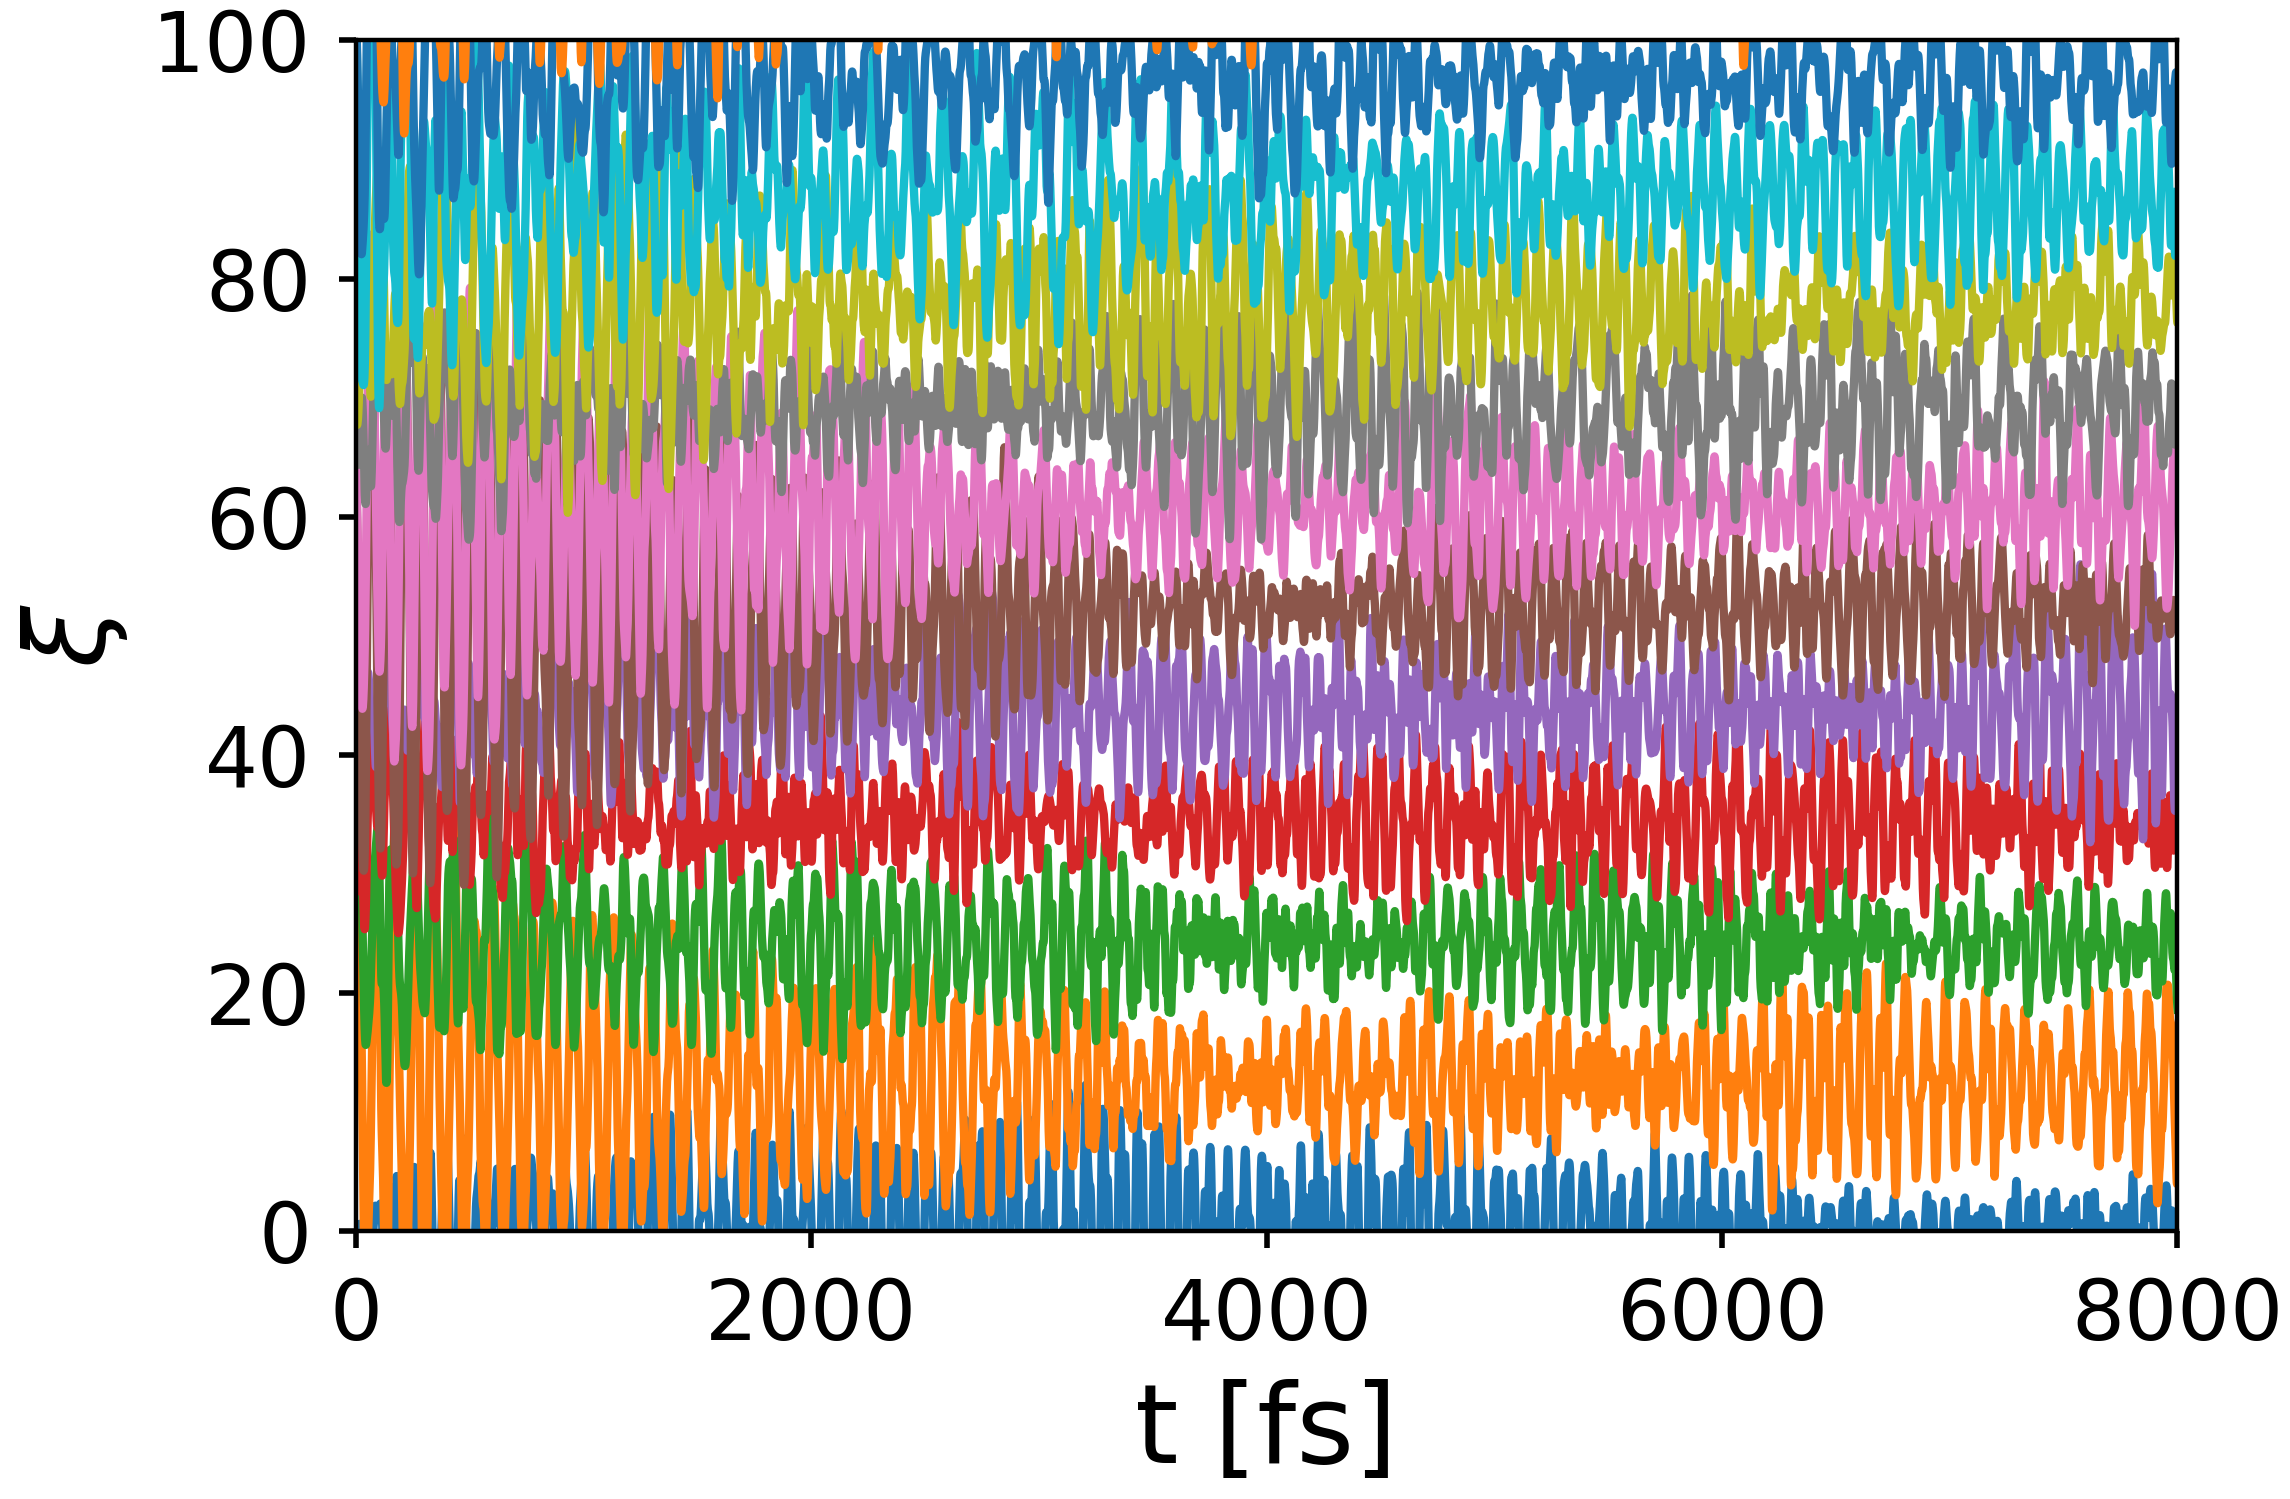
\includegraphics[width=0.7\textwidth]{bilder/traj} }}
%    \subfloat[]{{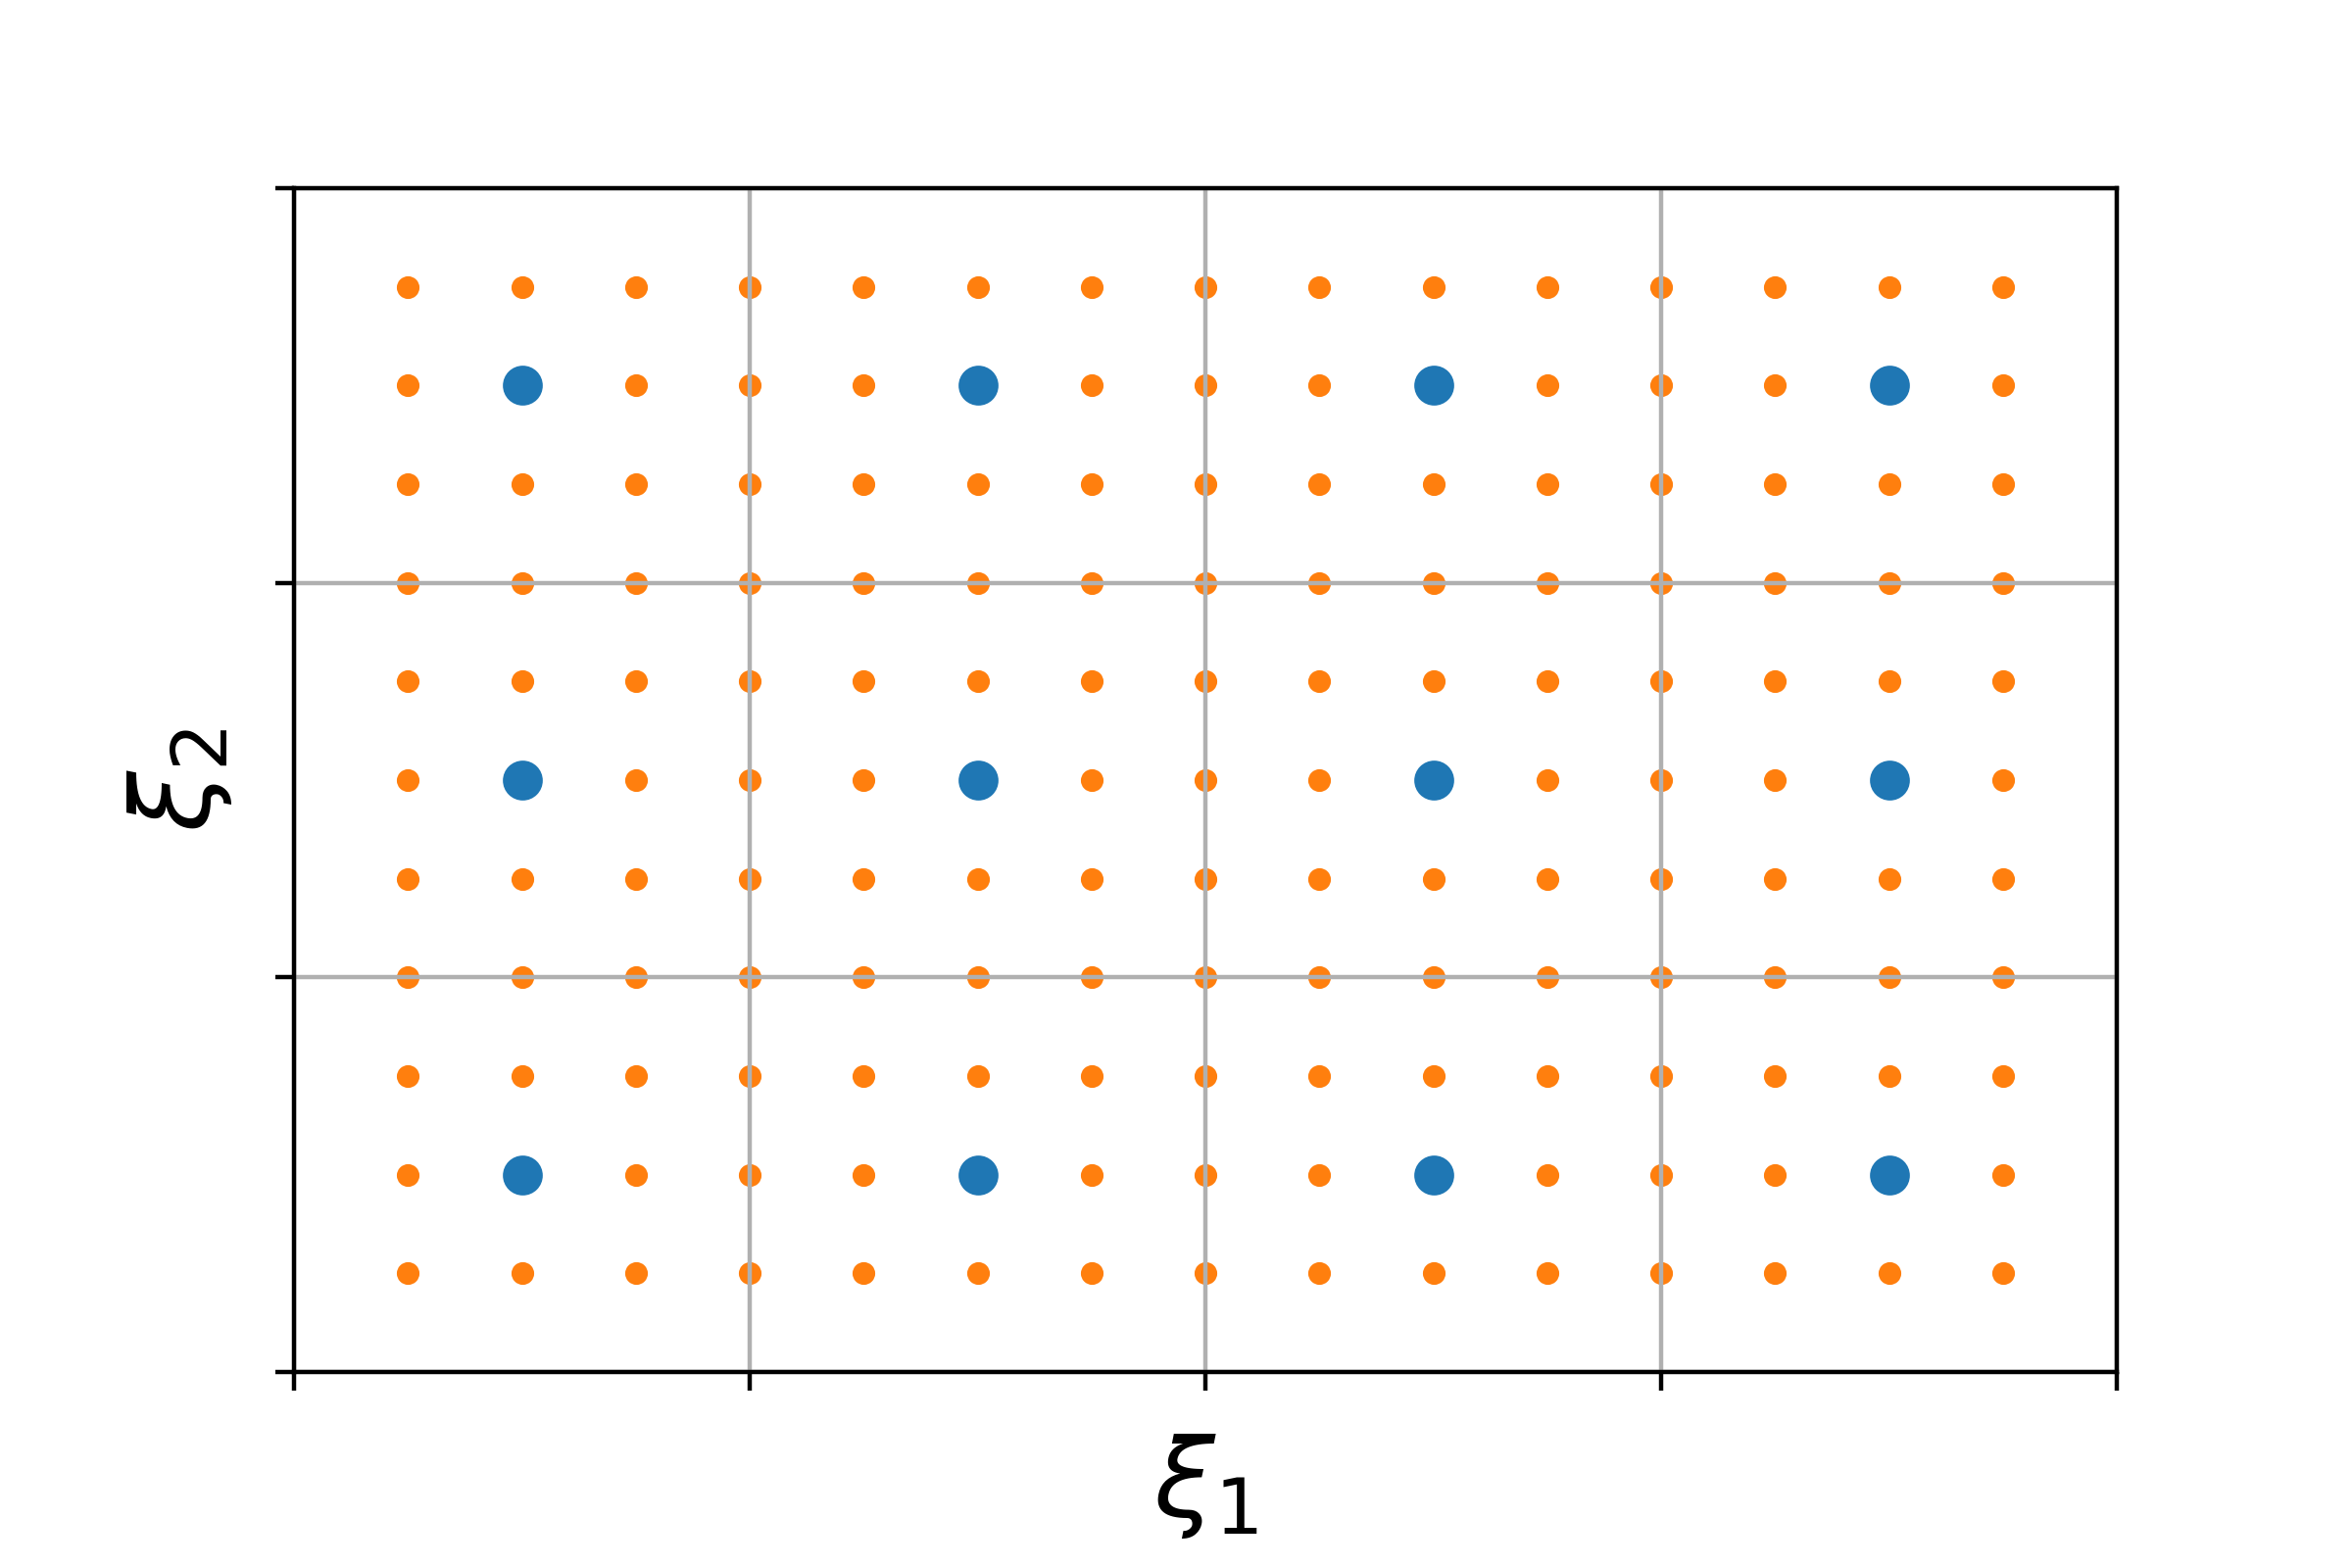
\includegraphics[width=0.5\textwidth]{bilder/grid} }}
%\label{fig:US}%
%\end{figure}

\newpage
\section{Adaptive Biasing Methods}
\label{sec:adaptive biasing}

Instead of dividing the reaction coordinate in several windows, with adaptive biasing methods the free energy can be estimated from one single simulation. For this purpose the systems dynamics are biased towards states corresponding to large values of the free energy along the transition coordinate via a history-dependent biasing potential. In contrast to other importance sampling strategies like umbrella sampling, this methods require no prior knowledge of the free-energy landscape at hand. Instead, the biasing potential automatically converges towards the free energy, enabling diffusive behavior along the transition coordinate.\autocite{comer2015adaptive, barducci2011metadynamics}

There are multiple adaptive biasing methods available, only differing in the construction of the bias. Potential based methods like metadynamics (MtD) disfavor already visited states by accumulating repulsive potentials along the CV (section \ref{sec:metaD}), while adaptive biasing force (ABF) methods compensate the mean force along the reaction coordinate to obtain uniform sampling (section \ref{sec:ABF}). Finally, as discussed in section \ref{sec:eABF}, using an extended Lagrangian, the technical requirements of ABF can be lifted without loosing its rigorous convergence behavior.\autocite{lesage2017smoothed} Additionally, this framework enables the combination of repulsive Mtd-potentials with ABF (meta-eABF/WTM-eABF), to unite the strengths of both approaches.\autocite{fu2018zooming,fu2019taming}

Although not necessary, stratification can increase the convergence of all adaptive biasing methods significantly. However, in contrast to US simulations, to combine windows WHAM is not required and no overlap between windows is required. For example in ABF simulations the global PMF can be recovered by simply joining the force estimates of all simulations.\autocite{comer2015adaptive} Multiple-Walker strategies can also be trivially implemented, by letting more than one simulation contribute to the same biasing potential.\autocite{minoukadeh2010potential}

In principle adaptive biasing methods only rely on sampling of the canonical ensemble, which will be obtained using Langevin dynamics in this work. However, all methods can also be applied in combination with other MD or MC engines. A schematic procedure of adaptively biased Langevin dynamics is given in Algorithm \ref{alg:ABM}.

\begin{algorithm}[H]
  \caption{Velocity Verlet integrator for adaptively biased Langevin dynamics with atomic masses $\textbf{M}$, coordinates $\textbf{x}(t)$, momenta $\textbf{p}(t)$, potential $V(\textbf{x}(t))$, forces $F(\textbf{x}(t))$ and friction coefficient $\gamma$,}
  \label{alg:ABM}
    \begin{algorithmic}
      \WHILE{$t < t_{end}$}
        \STATE
        \STATE $\textbf{p}(t+\frac{1}{2}\Delta t) \leftarrow \textbf{p}(t) + \frac{1}{2} \bigl(F(\textbf{x}(t))dt-\gamma \textbf{M}^{-1}\textbf{p}(t) dt + \sqrt{2\gamma\beta^{-1}}dW_t \bigr)$
        \STATE $\textbf{x}(t+\Delta t) \leftarrow \textbf{x}(t) + \frac{2}{2+\gamma dt}\textbf{M}^{-1} \textbf{p}(t+\frac{1}{2}\Delta t) dt$
        \STATE /* Langevin dynamics
        \STATE
        \STATE $F(\textbf{x}(t+\Delta t)) \leftarrow -\nabla U(\textbf{x}(t+\Delta t))$
        \STATE /* get physical QM/MM forces
        \STATE
        \STATE $\xi \leftarrow f(\textbf{x}(t+\Delta t))$
        \STATE /* Calculate reaction coordinate from Cartesian coordinates
        \STATE
        \IF{$\xi_{min}\leq\xi\leq\xi_{max}$}
          \STATE
          \STATE $F_{B}(\xi, t+\Delta t))\leftarrow F_{B}(\xi, t))+\Delta F_{B}(\xi,t+\Delta t))$
          \STATE /* update history dependent bias force along reaction coordinate incrementally
          \STATE
          \STATE $F(\textbf{x}(t+\Delta t)) \leftarrow -\nabla U(\textbf{x}(t+\Delta t)) + F_{B}(\xi, t+\Delta t))\nabla\xi$
          \STATE /* Add biasing force to physical force
          \STATE
        \ELSE
          \STATE
          \STATE $F(\textbf{x}(t+\Delta t)) \leftarrow F(\textbf{x}(t+\Delta t)) + k\min(|\xi-\xi_{min}|,|\xi-\xi_{max}|)\nabla\xi$
          \STATE /* confine system to range of interest with harmonic constraining force
          \STATE
        \ENDIF
        \STATE
        \STATE $\textbf{p}(t+\Delta t) = \frac{2 - \gamma dt}{2+\gamma dt} \textbf{p}(t+\frac{1}{2}\Delta t) - \frac{1}{2} \bigl(F(\textbf{x}(t+\Delta t))dt-\gamma \textbf{M}^{-1}\textbf{p}(t+\frac{1}{2}\Delta t)) dt + \sqrt{2\gamma\beta^{-1}}dW\bigr)$
        \STATE /* Langevin dynamics
        \STATE
      \ENDWHILE
      \STATE /* get unbiased free energy
    \end{algorithmic}
\end{algorithm}

\newpage
\subsection{(Well-Tempered) Metadynamics (MtD/WTM)}
\label{sec:metaD}

MetaD biases a systems dynamic towards under-sampled regions along the reaction coordinate $\xi(\textbf{x})$, by accumulating repulsive potentials in regions that have already been visited. The bias potential is typically build by a superposition of repulsive Gaussian kernels and can be written:\autocite{barducci2011metadynamics}
\begin{equation}
  U_{MtD}(\xi,t)= \sum_{k<\frac{t}{\tau_G}} \tau_G \omega \exp\biggr(-\sum_{i=1}^{N_{dim}} \frac{1}{2\sigma_{i}^{2}} (\xi_{i}(\textbf{x})-\xi_{i}(\textbf{x},t_k))^2 \biggl)
  \label{eq:U_mtD}
\end{equation}
with deposition rate $\tau_G$, Gaussian height $\omega=W/\tau_G$ and variance $\sigma^2$ as free input parameters. Over the course of a simulation the bias potential fills local minima along the reaction coordinate until the systems evolution finally resembles a Brownian motion along the flattened free energy surface. The converged bias potential provides an unbiased estimate of the underlying free energy surface
\begin{equation}
  A(\xi) = -U_{MtD}(\xi, t \to \infty) + C
\end{equation}
To avoid oscillation of $U_{MtD}$ around the correct free energy, Well-Tempered metadynamics (WTM) introduces an additional scaling factor of the Gaussian height:\autocite{barducci2008well}
\begin{equation}
  \omega(\xi,t) = \frac{W}{\tau_G}\exp\biggl(-\frac{U_{WTM}(\xi,t)}{k_B \Delta T} \biggr)
  \label{eq:WTM}
\end{equation}
ensuring an decrease of $\omega$ over time and smooth convergence of the Well-Tempered bias potential $U_{WTM}(\xi,t)$. The WTM bias potential does not fully compensate the free energy surface, but can be controlled by parameter $\Delta T$. For $\Delta T \to 0$ the bias is zero and ordinary MD is recovered, whereas the limit $\Delta T \to \infty$ corresponds to normal metaD. Figure~\ref{fig:metaD} show a numerical example of the effect of $U_{mtD}$ and $U_{WTM}$ on the effective free energy energy surface over the course of a simulation.

\begin{figure}[H]
    \centering
    \subfloat[Metadynamics]{{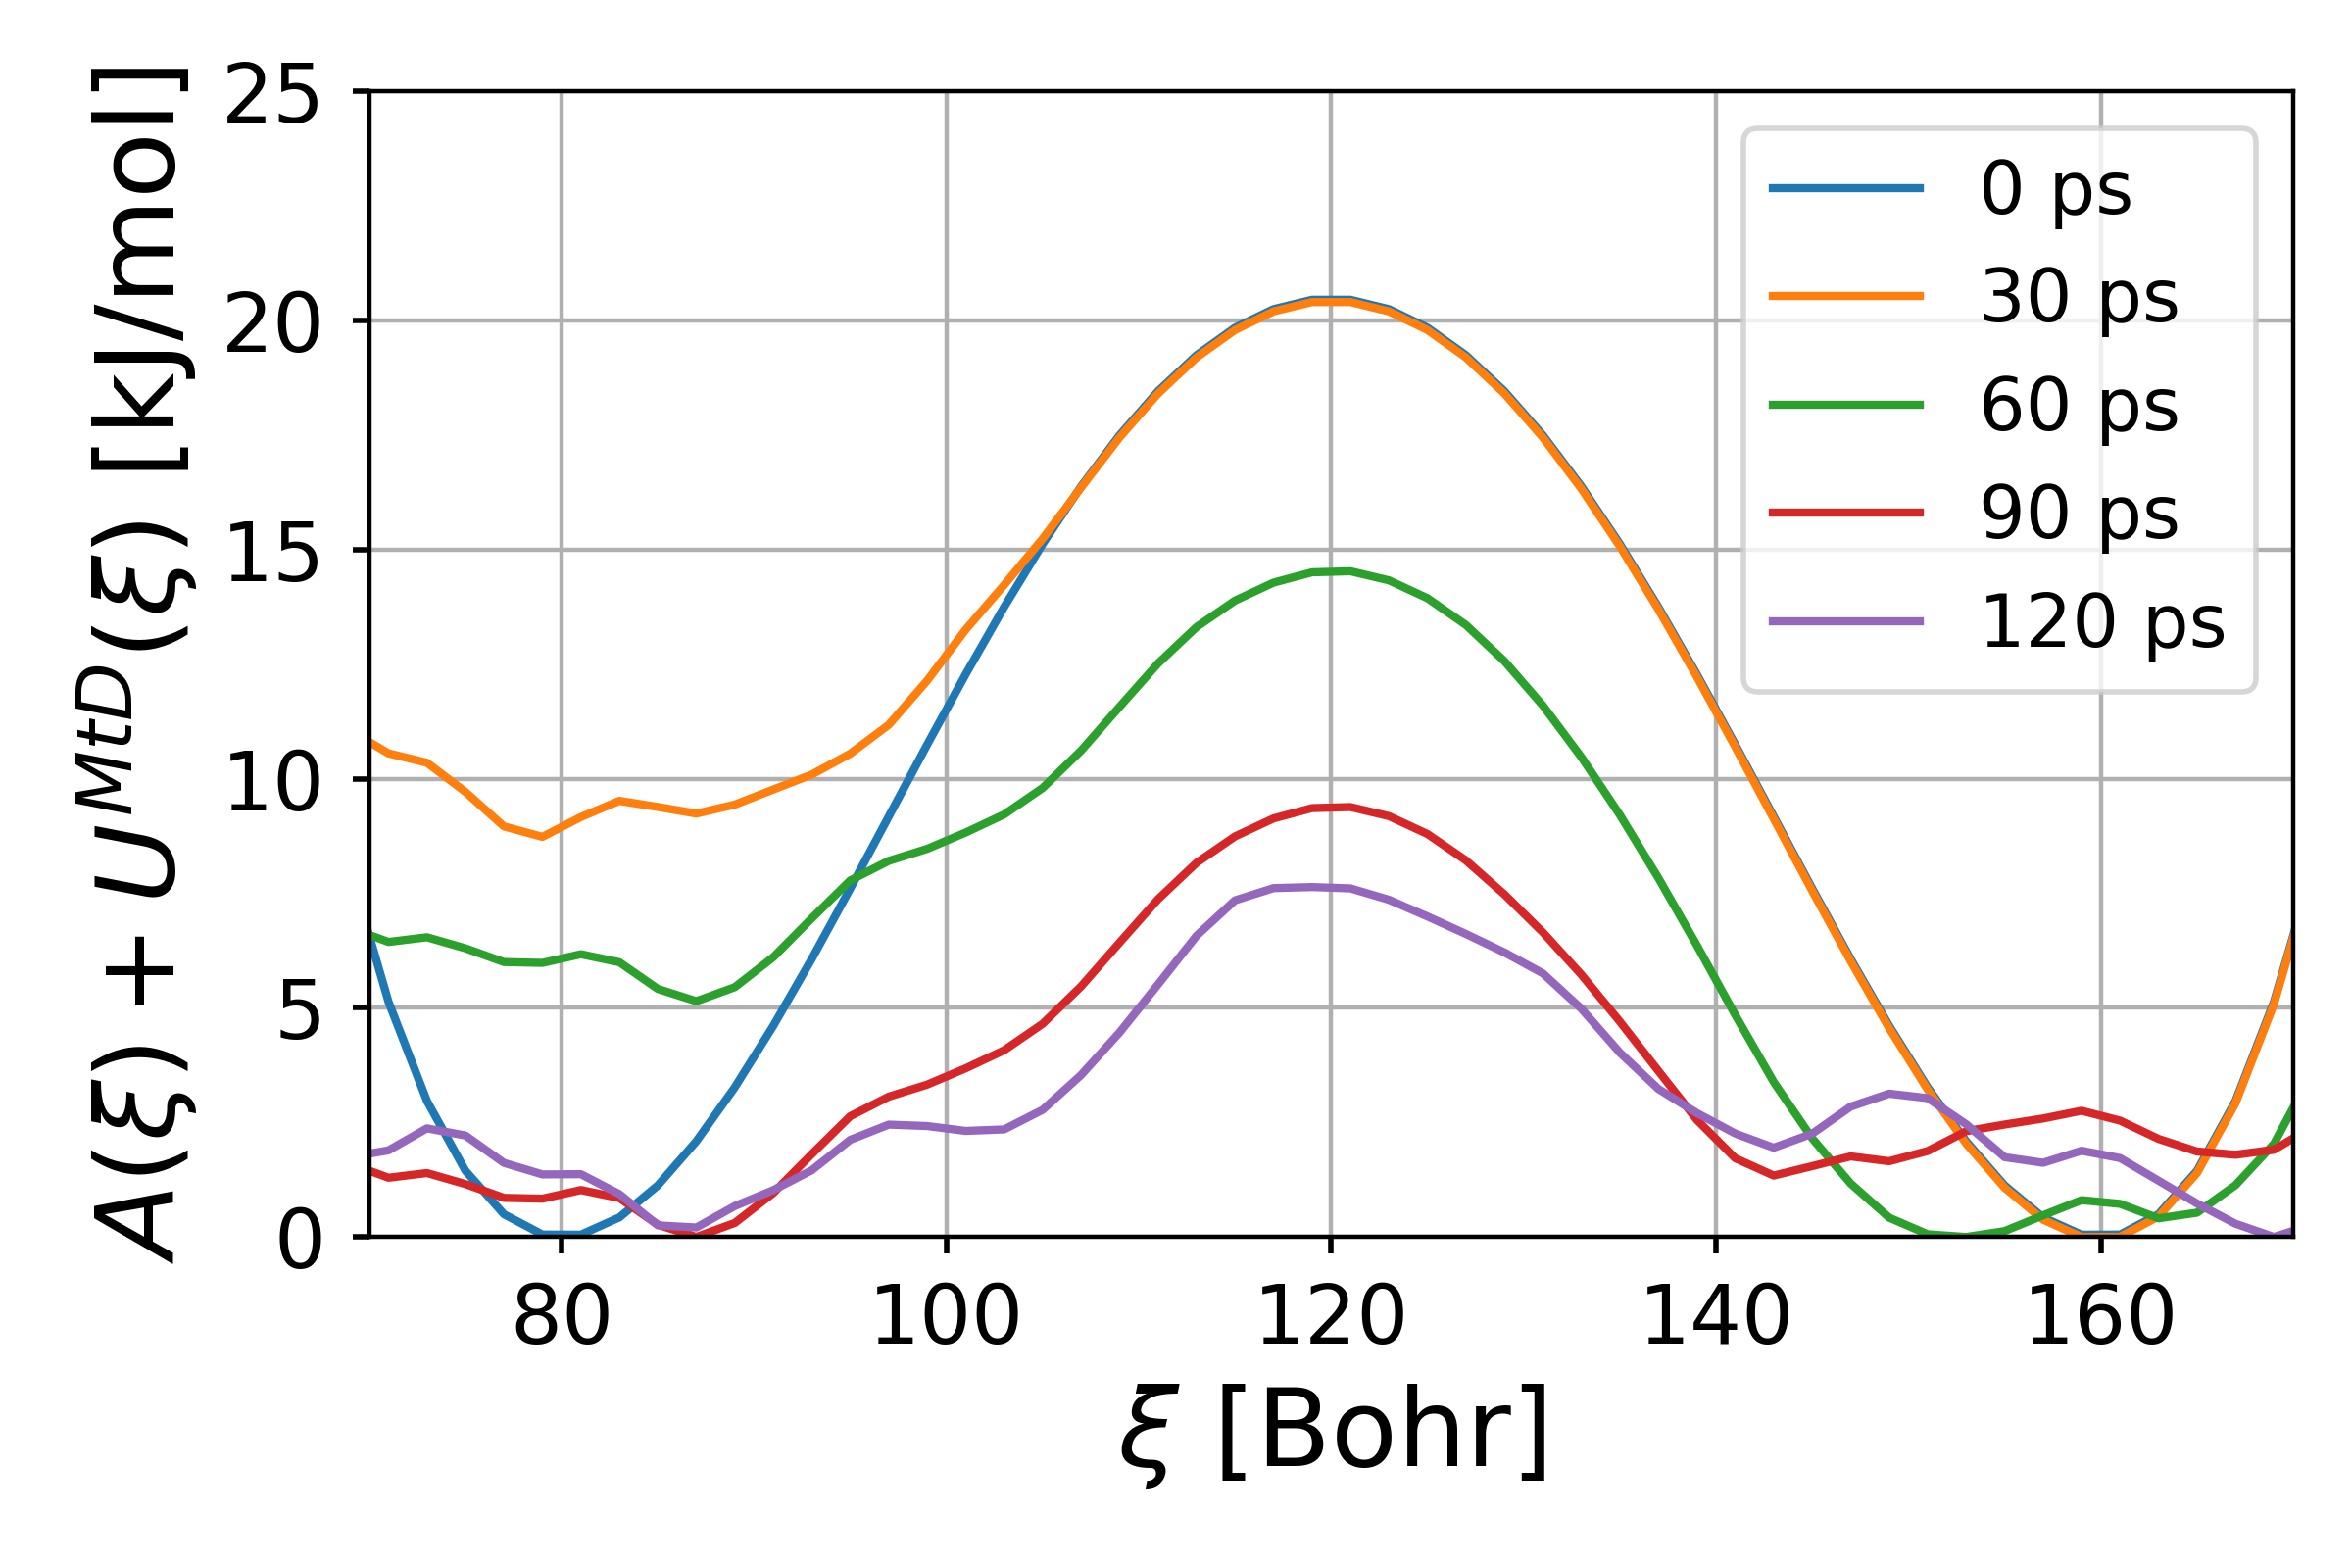
\includegraphics[width=0.49\textwidth]{bilder/metaD_eff_pot} }}
    \subfloat[Well-Tempered Metadynamics]{{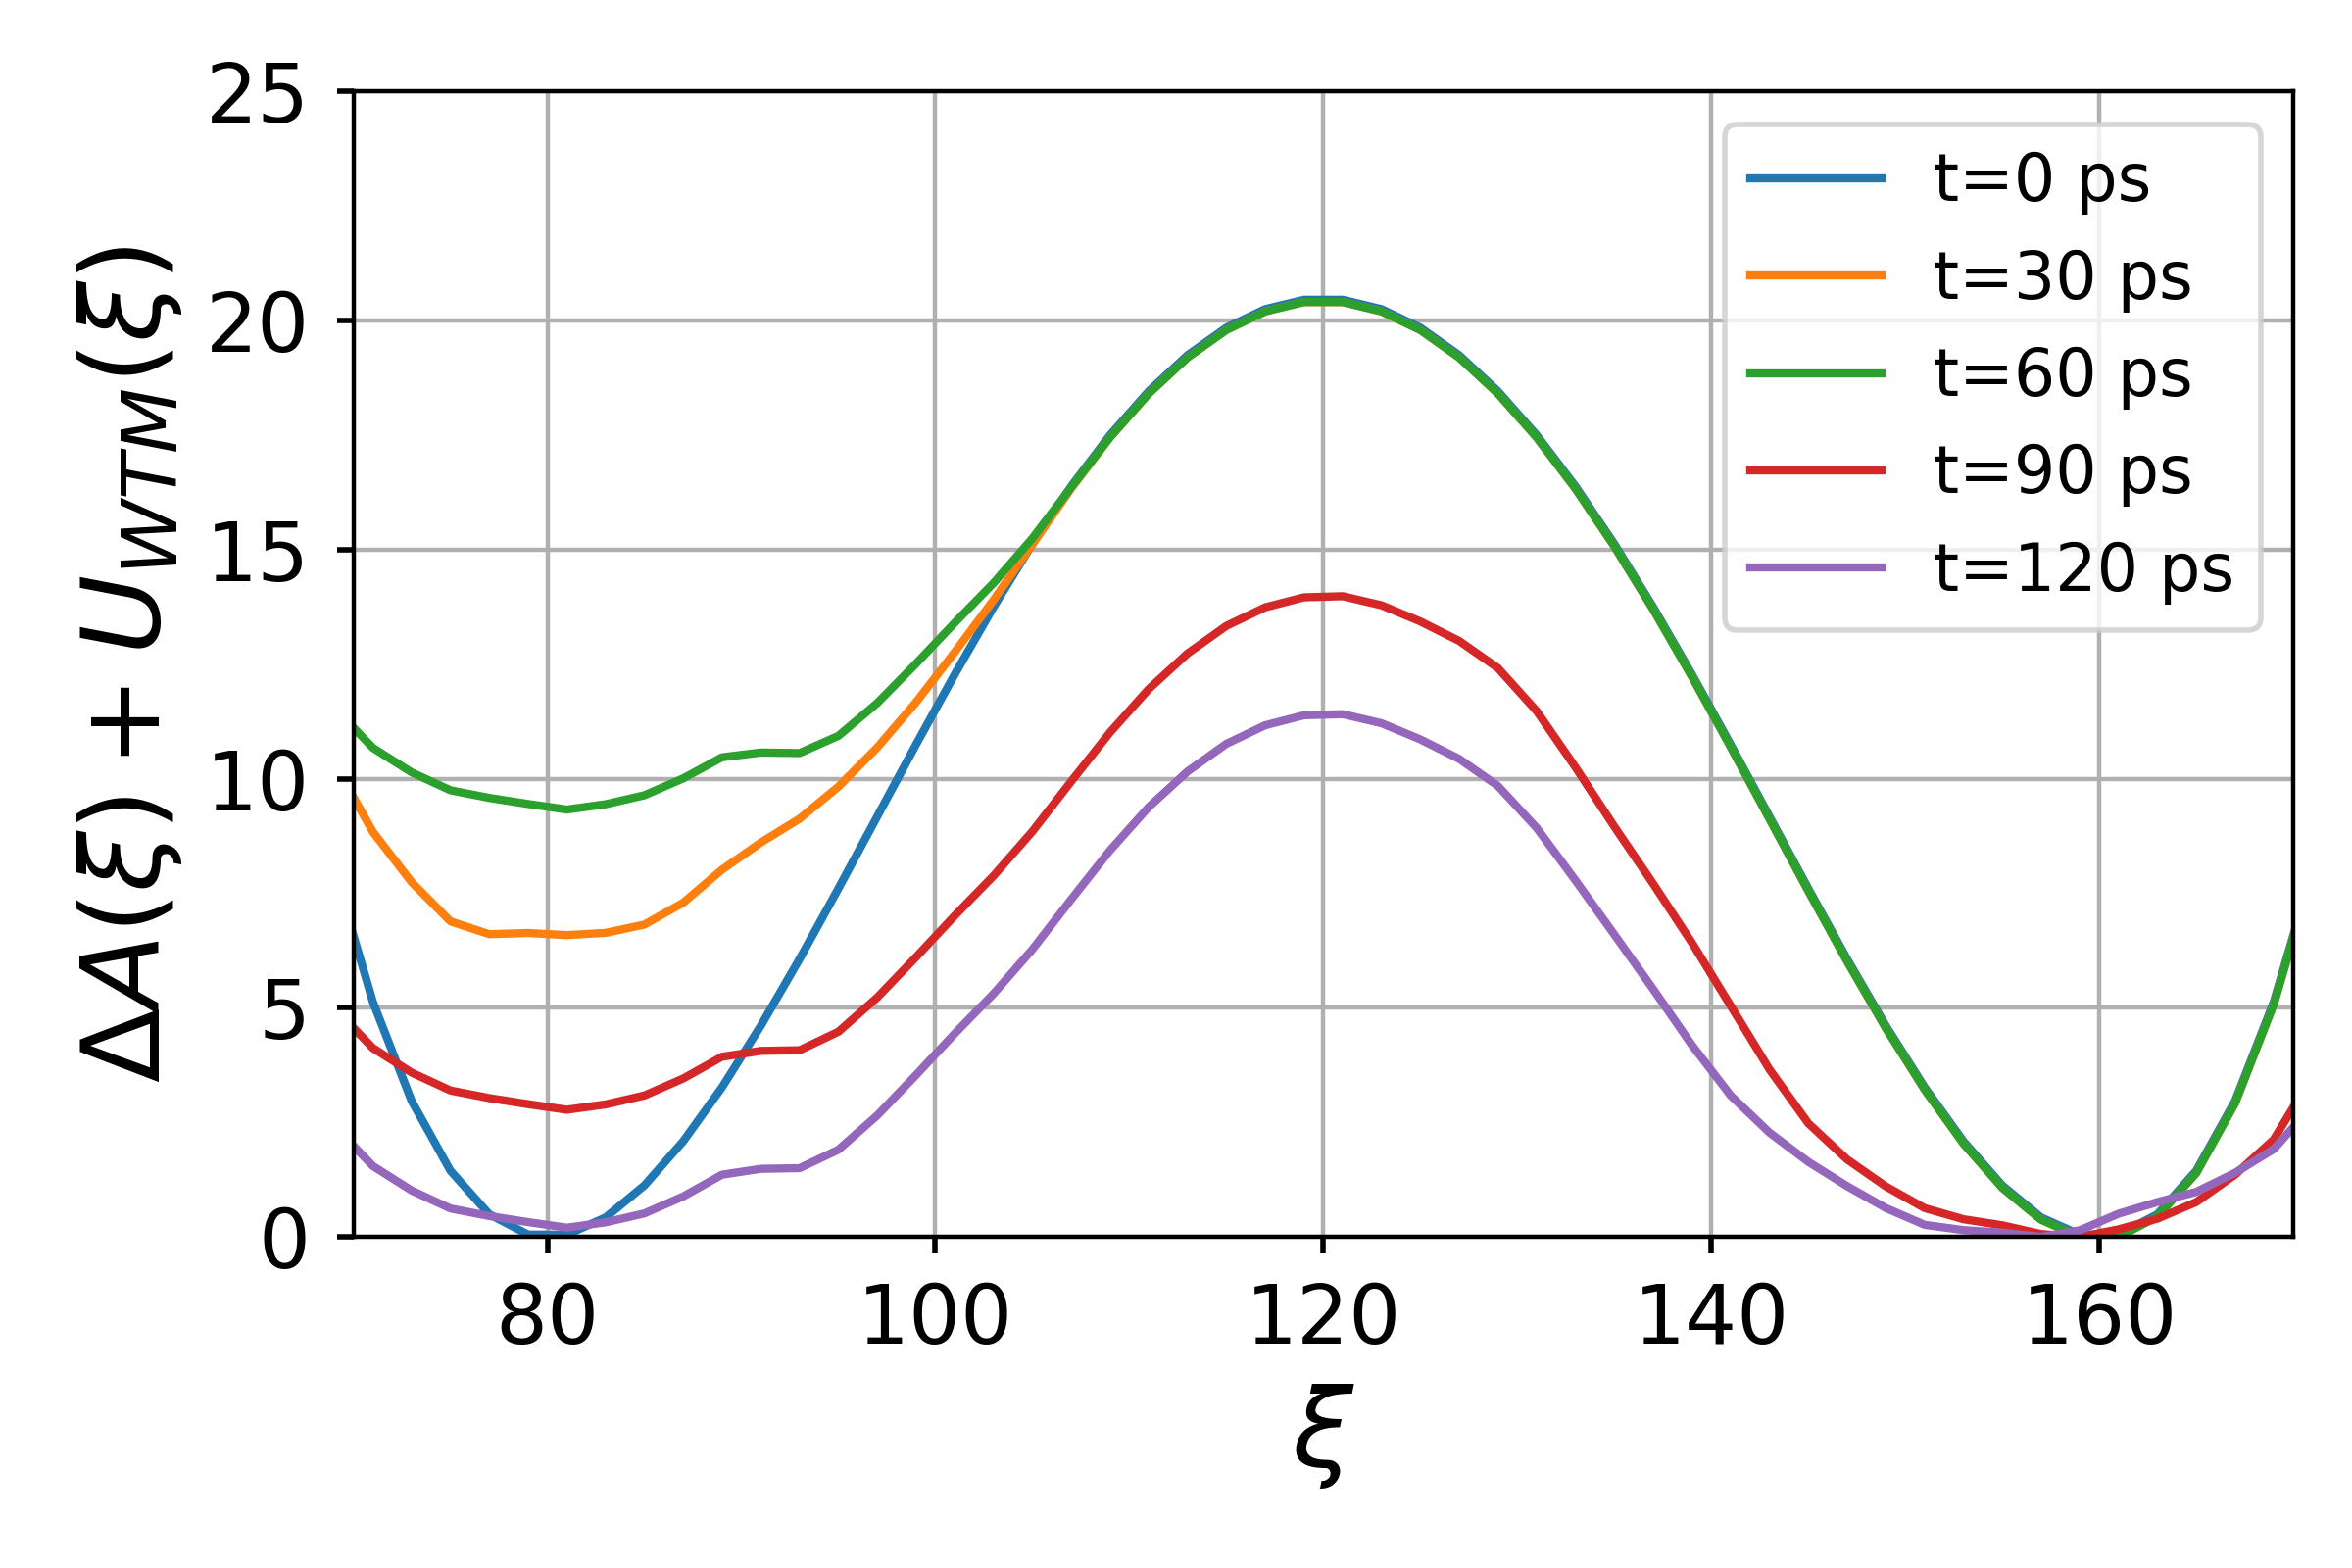
\includegraphics[width=0.49\textwidth]{bilder/WTM_eff_pot} }}
    \caption{Numerical example of metaD and WTM algorithm for 2D double well potential. The reaction coordinate $\xi$ is the x-direction. Over time the bias potentials $U_{MtD}$ and $U_{WTM}$ build up and reduce the free energy barrier. $U_{MtD}$ will ultimately completely remove the free energy barrier, whereas $U_{WTM}$ converges to a certain limit, which can be controlled with parameter $\Delta T$. Details are given in the Appendix.}
\label{fig:metaD}%
\end{figure}

To again obtain the unbiased PMF from $U_{WTM}(\xi,t)$ it has to be scaled with an according correction factor to compensate the effect of $\Delta T$:
\begin{equation}
A(\xi) = -\frac{T+\Delta T}{\Delta T}U_{WTM}(\xi, t)
\end{equation}
Despite its appealing theoretical and practical simplicity metaD and WTM both suffer from the rather big set of parameters that have to be chosen prior to the simulation. All of them have significant impact on the outcome of the simulation and are not trivial to chose. If the bias potential builds up too fast the system is driven far away from equilibrium and the obtained free energy estimate is wrong. Small parameters on the other hand result in bad convergence behavior and inefficient sampling.\autocite{laio2005assessing}
The next section will look into ABF, which is less dependent on free parameters and stands on a more rigorous mathematical framework.

\newpage
\subsection{Adaptive Biasing Force Method (ABF)}
\label{sec:ABF}

The intuition behind ABF is, that adding a force $A'(\xi(\textbf{x}))\nabla\xi(\textbf{x})$ that exactly compensates the average of the original force $-\nabla U(\textbf{x})$ along a given coordinate would result in uniform sampling along this coordinate.\autocite{comer2015adaptive}
Historically, this idea emerged from thermodynamic integration (TI), were the free energy derivative  is computed as the ensemble average of the instantaneous force, $F$, acting along the collective variable:
\begin{equation}
\frac{dA}{d\xi} = -\braket{F}_{\xi}
\end{equation}
and the free energy is calculated as the integral over this force.\autocite{kirkwood1935statistical,zwanzig1954high}
In practice, as one has no prior knowledge of the free energy derivative, ABF uses an on-the-fly estimate of the mean force acting along the reaction coordinate. For this purpose the transition coordinate $\xi$, connecting two end points, is divided in $M$ equally spaced bins. The approximation of the bias force $\overline{F}(N_{Step},k)$ in bin $k$ is than the average of all collected force samples:\autocite{comer2015adaptive}
\begin{equation}
  \overline{F}(N_{Step},k) = \frac{1}{N_{Step}^{k}} \sum_{\mu=1}^{N_{Step}^{k}} F_{\mu}^{k}
  \label{eq:mean force}
\end{equation}
At the beginning of the simulation the applied bias force is scaled up by a linear ramp function $R(N_{step}^k,k)$ to prevent large fluctuations of the force estimate from driving the system away from equilibrium.
\begin{equation}
  R(N_{step}^k,k)=\left\{\begin{array}{ll} N_{full}, & N_{step}^{k} < N_{full} \\
                                         1,  & N_{step}^{k} \geq  N_{full} \end{array}\right. \label{eq:ramp}
\end{equation}
The number of samples when the full biasing force is applied, $N_{full}$, and the bin size are the only free parameters that have to be chosen by the user before the simulation.
It can be proven mathematically, that \ref{eq:mean force} converges (under some constraints even exponentially) to $-dA/d\xi$ for a sufficiently large number of force samples.\autocite{alrachid2015long}
Figure~\ref{fig:ABF} shows a numerical example for the flattening of the reaction coordinate during an ABF simulation.

\begin{figure}[H]
    \centering
    \vspace{-1cm}
    \subfloat[ABF force $\overline{F}$]{{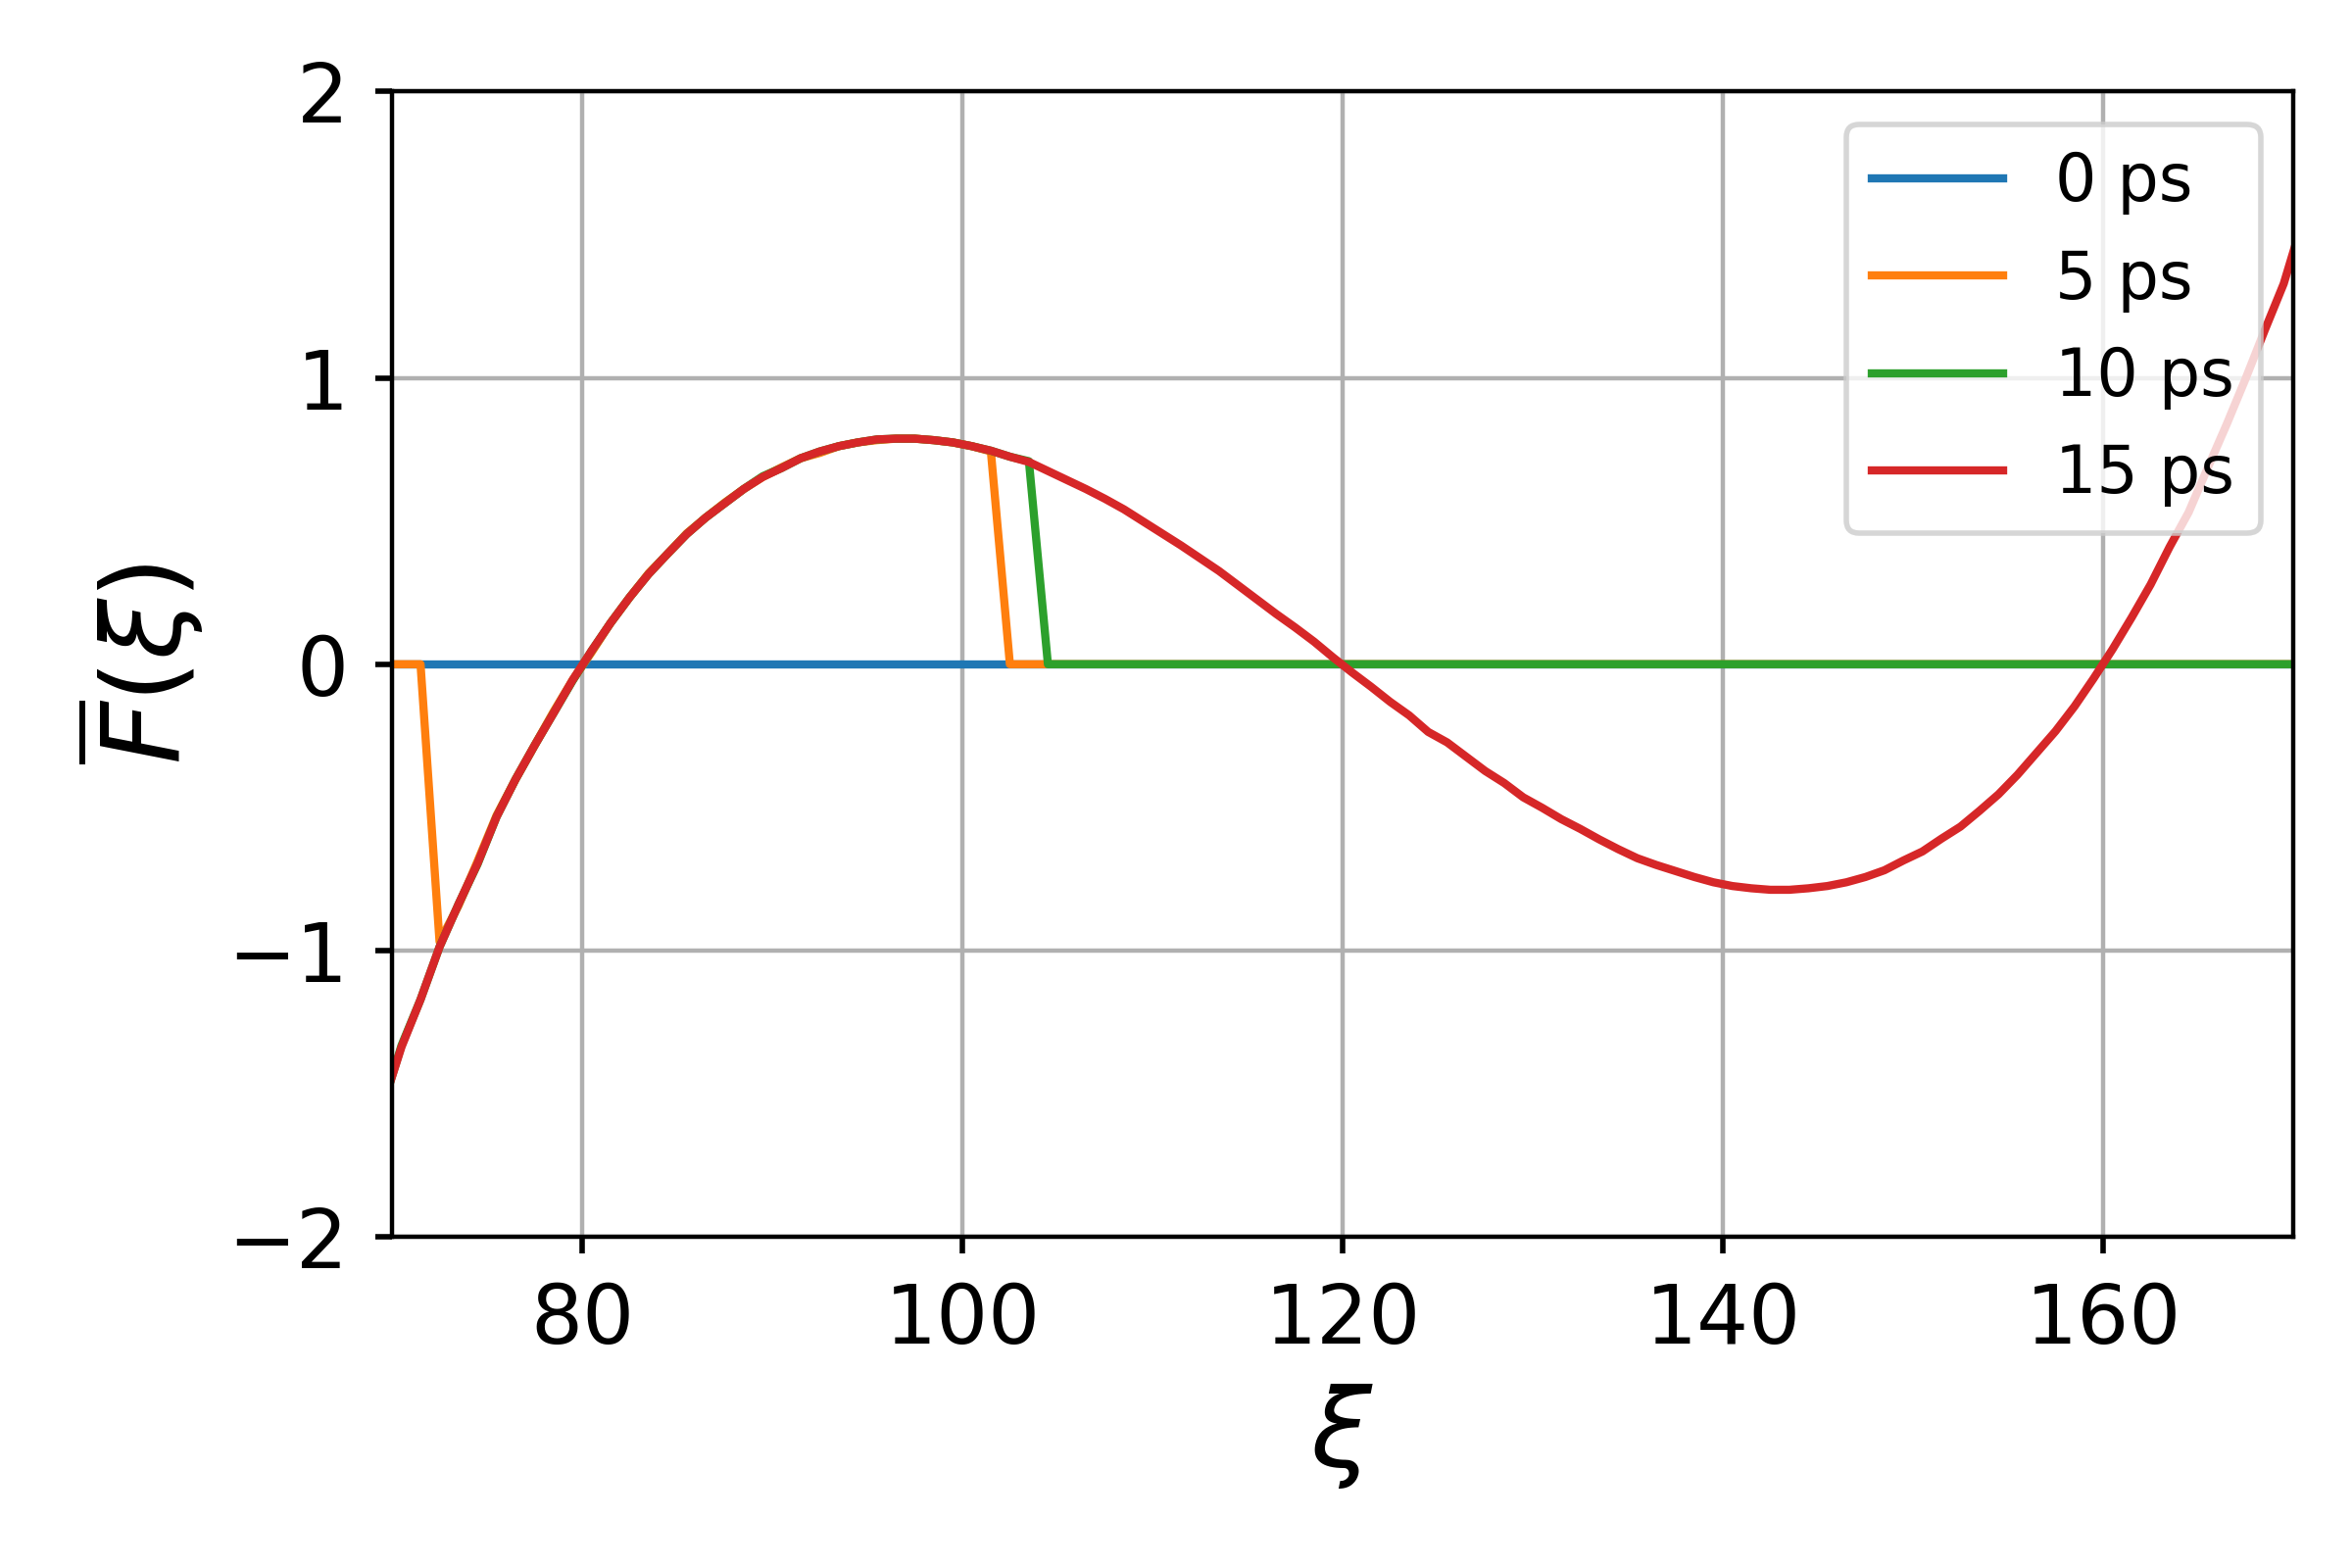
\includegraphics[width=0.49\textwidth]{bilder/ABF_force} }}
    \subfloat[effective potential ($A(\xi)-\int\overline{F}(\xi)d\xi$) during ABF simulation ]{{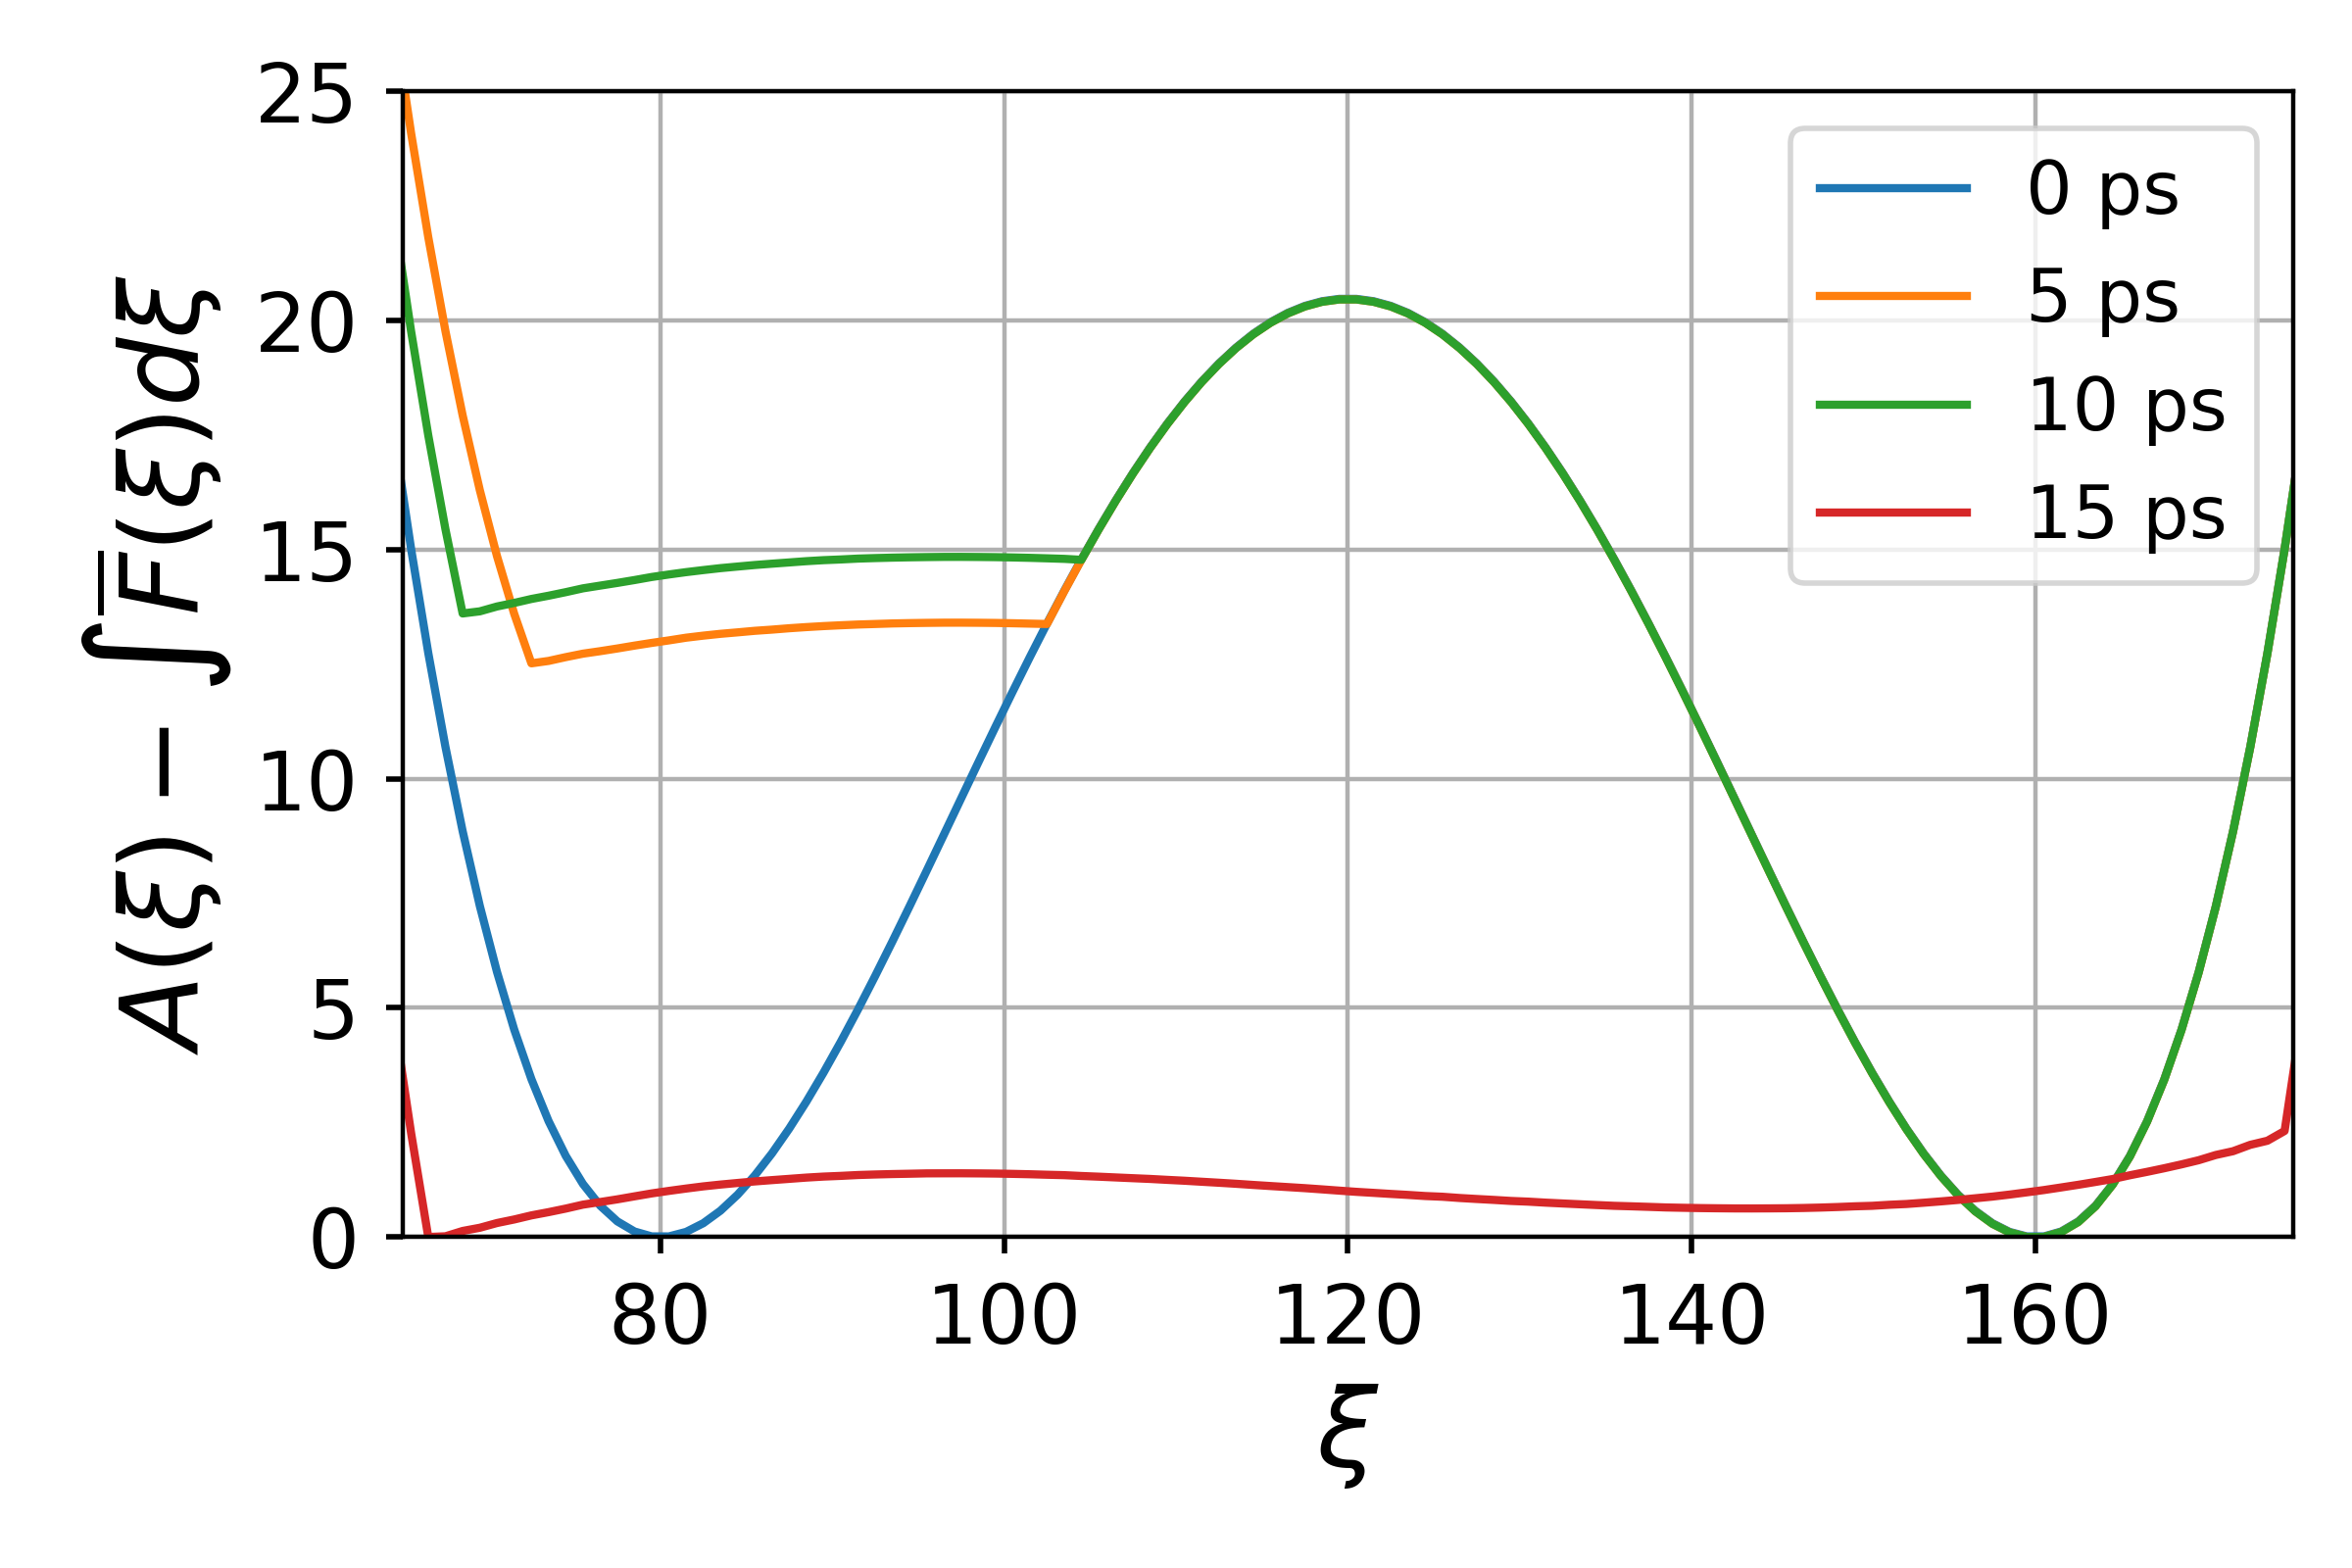
\includegraphics[width=0.49\textwidth]{bilder/ABF_freeE} }}
    \caption{Numerical example of ABF algorithm for 2D double well potential. The reaction coordinate $\xi$ is the x-direction. $\overline{F}(\xi)$ completely compensates the free energy barrier after 15~ps. From there on the system evolution resembles Brownian motion along the flattened reaction coordinate, which will ultimately lead to uniform sampling. Details are given in the Appendix.}
\label{fig:ABF}%
\end{figure}

For 1D reaction coordinates the unbiased free energy difference $\Delta A$ can be trivially obtained from $\overline{F}$ with any numerical integration scheme (e.g. Simpson's rule).
However, this is not true for multidimensional reaction coordinates, because $\overline{F}$ is no conservative force due to statistical errors. With simple integration the result would therefore depend on the integration path, which is physically wrong. This problem can be avoided by using the finite element method (FEM). For this purpose tent functions $B_l$ are used to approximate $A(\xi)$:\autocite{darve2008adaptive}
\begin{equation}
  A(\xi) = \sum_l \alpha_l B_l(\xi)
\end{equation}
where the coefficients $\alpha_l$ are obtained by minimizing
\begin{equation}
  RMSD(\vec{\alpha})=\sqrt{\frac{1}{M}\sum_k^M\biggl(\bigl(\sum_l \alpha_l \nabla B_l(\xi_k)\bigr) - \braket{F(\xi_k)} \biggr)^2}
\end{equation}
with some numerical minimization routine (e.g. BFGS algorithm\autocite{nocedal2006numerical}) for force estimates of each dimension simultaneously. An 1D example of the approximation of an arbitrary function by tent functions is given in \ref{fig:FEM}a. To increase the smoothness of the reconstructed free energy surface in practice four control points per bin and dimension are chosen between data points, as shown in figure \ref{fig:FEM}b.

\begin{figure}[H]
    \centering
    \vspace{-1cm}
    \subfloat[Example of 1D tent functions $B_l(\xi)$ (colored) approximating an arbitrary free energy surface $f(\xi)$ (blue)]{{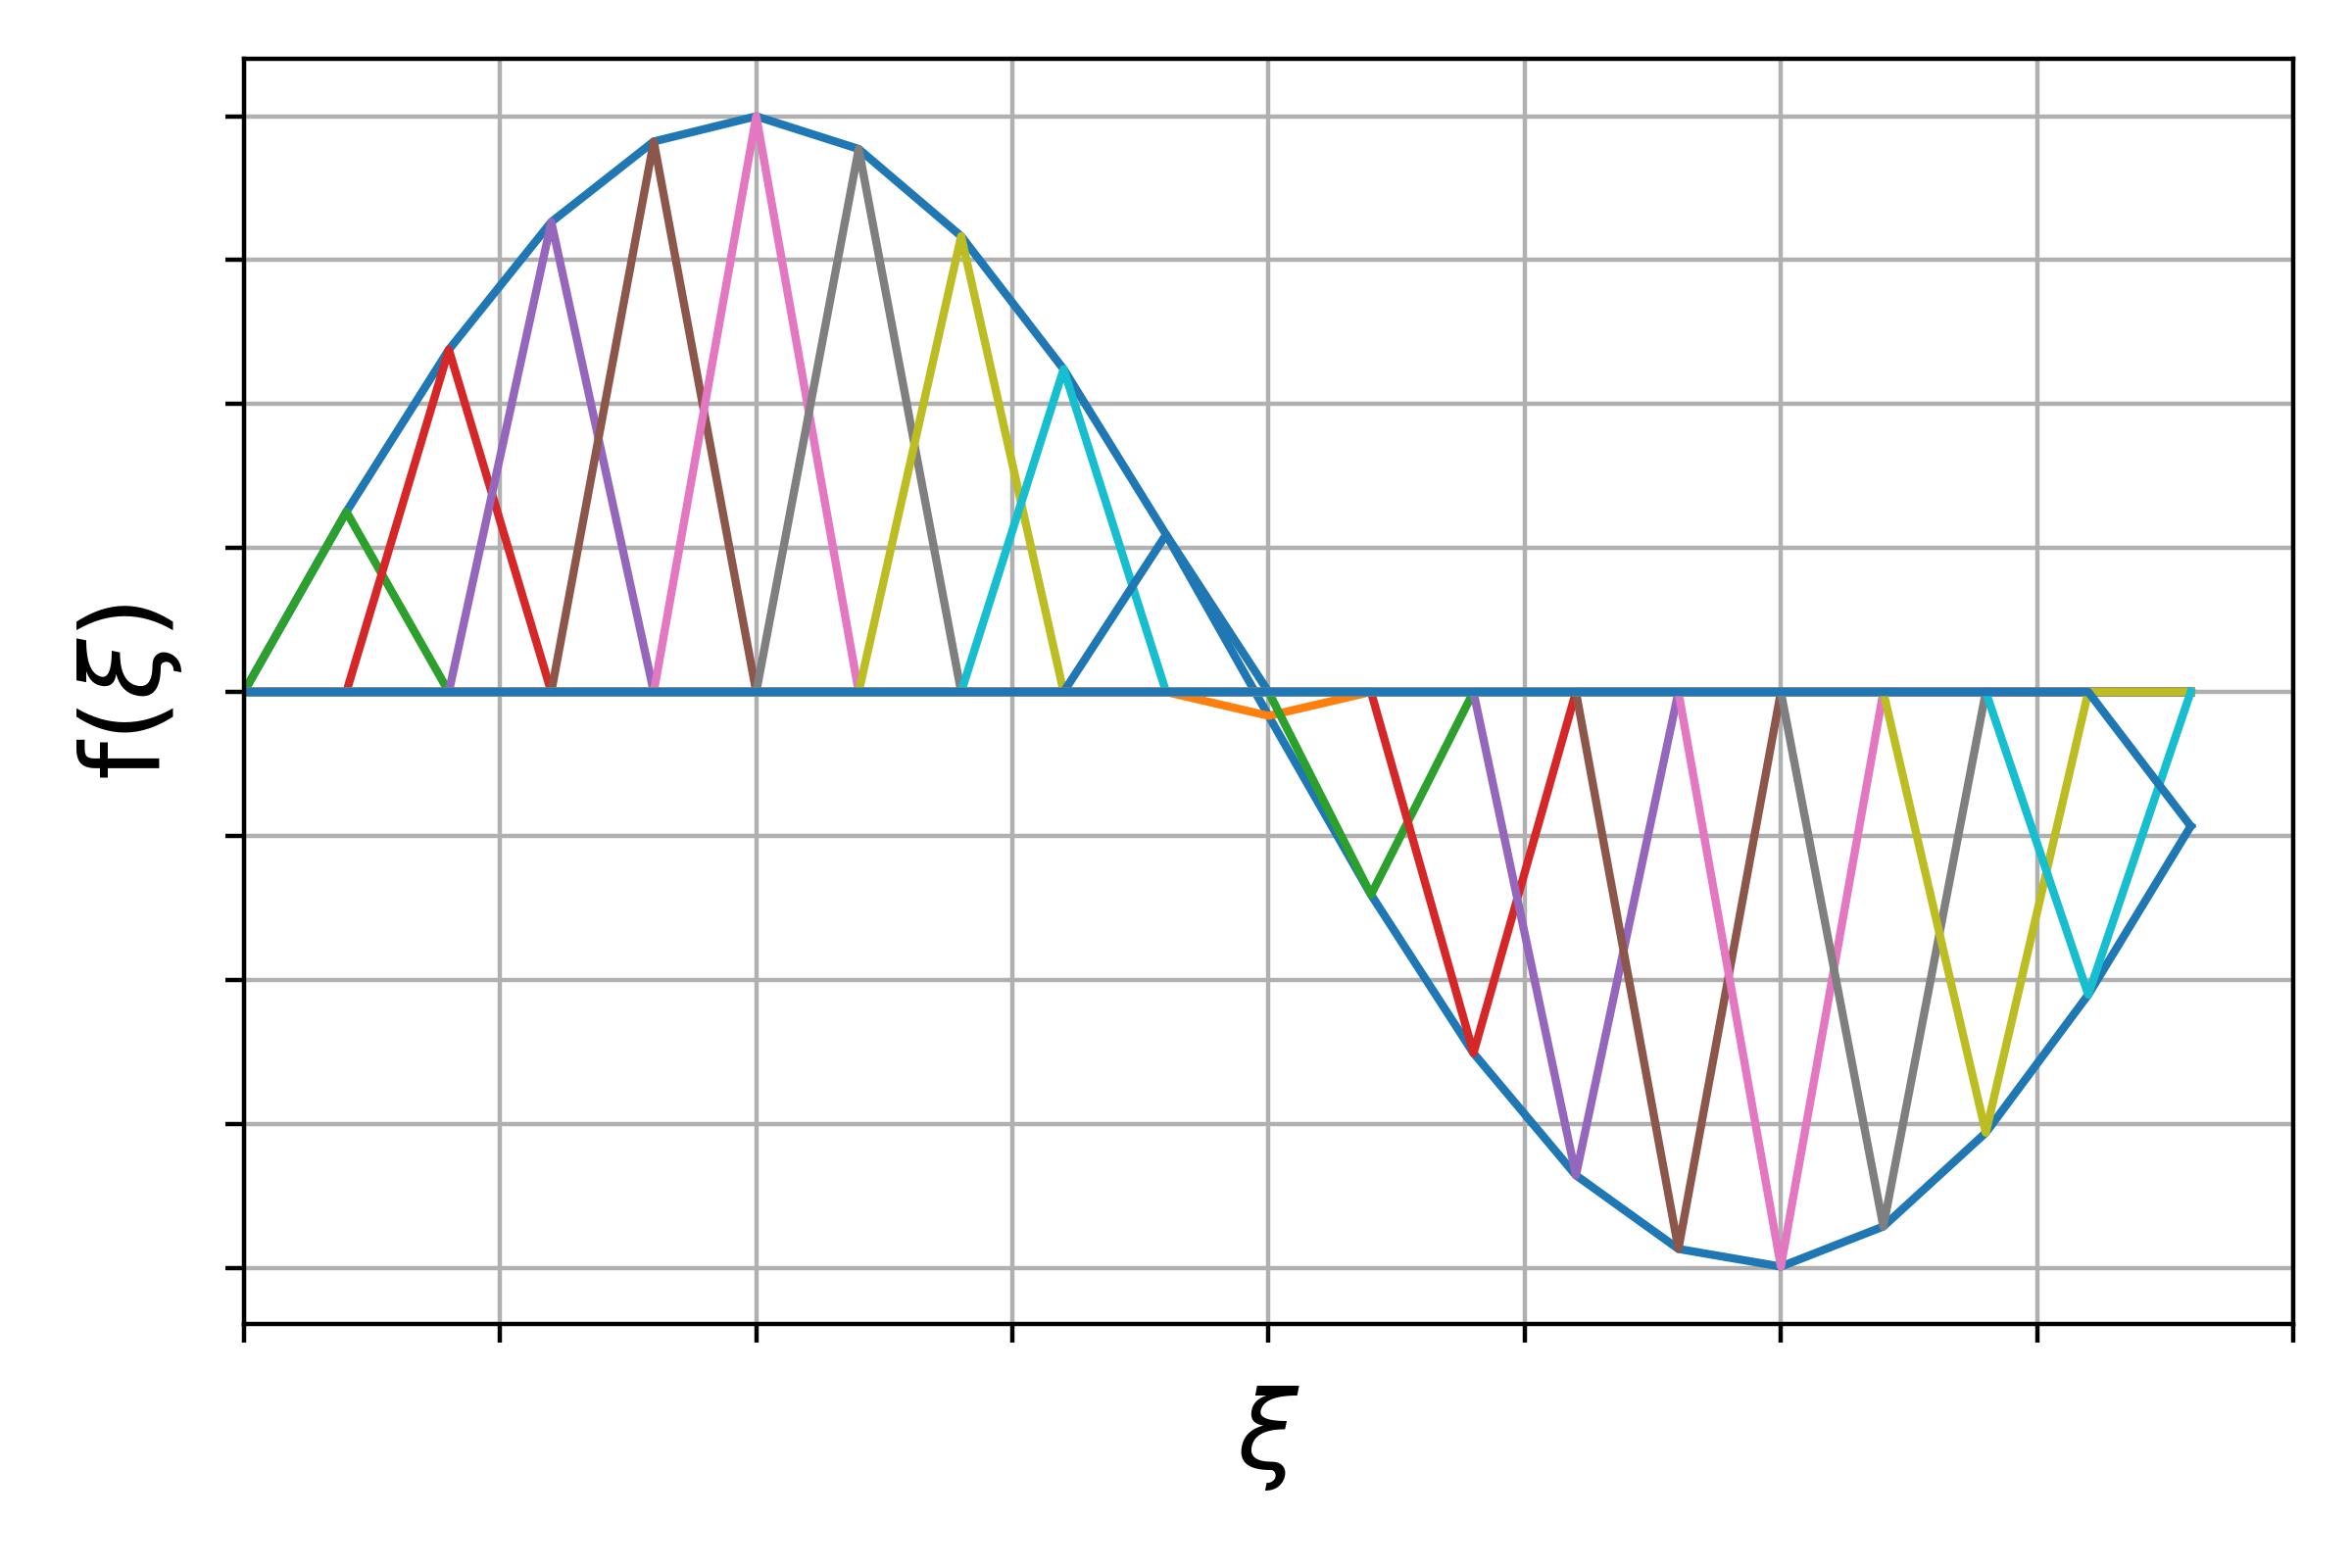
\includegraphics[width=0.44\textwidth]{bilder/FEM_1D} }}
    \subfloat[Illustration of numerical grid used for FEM integration of ABF-forces in 2D. Blue are original data points and orange control points obtained by linear interpolation. One 2D tent function is centered on each blue point.]{{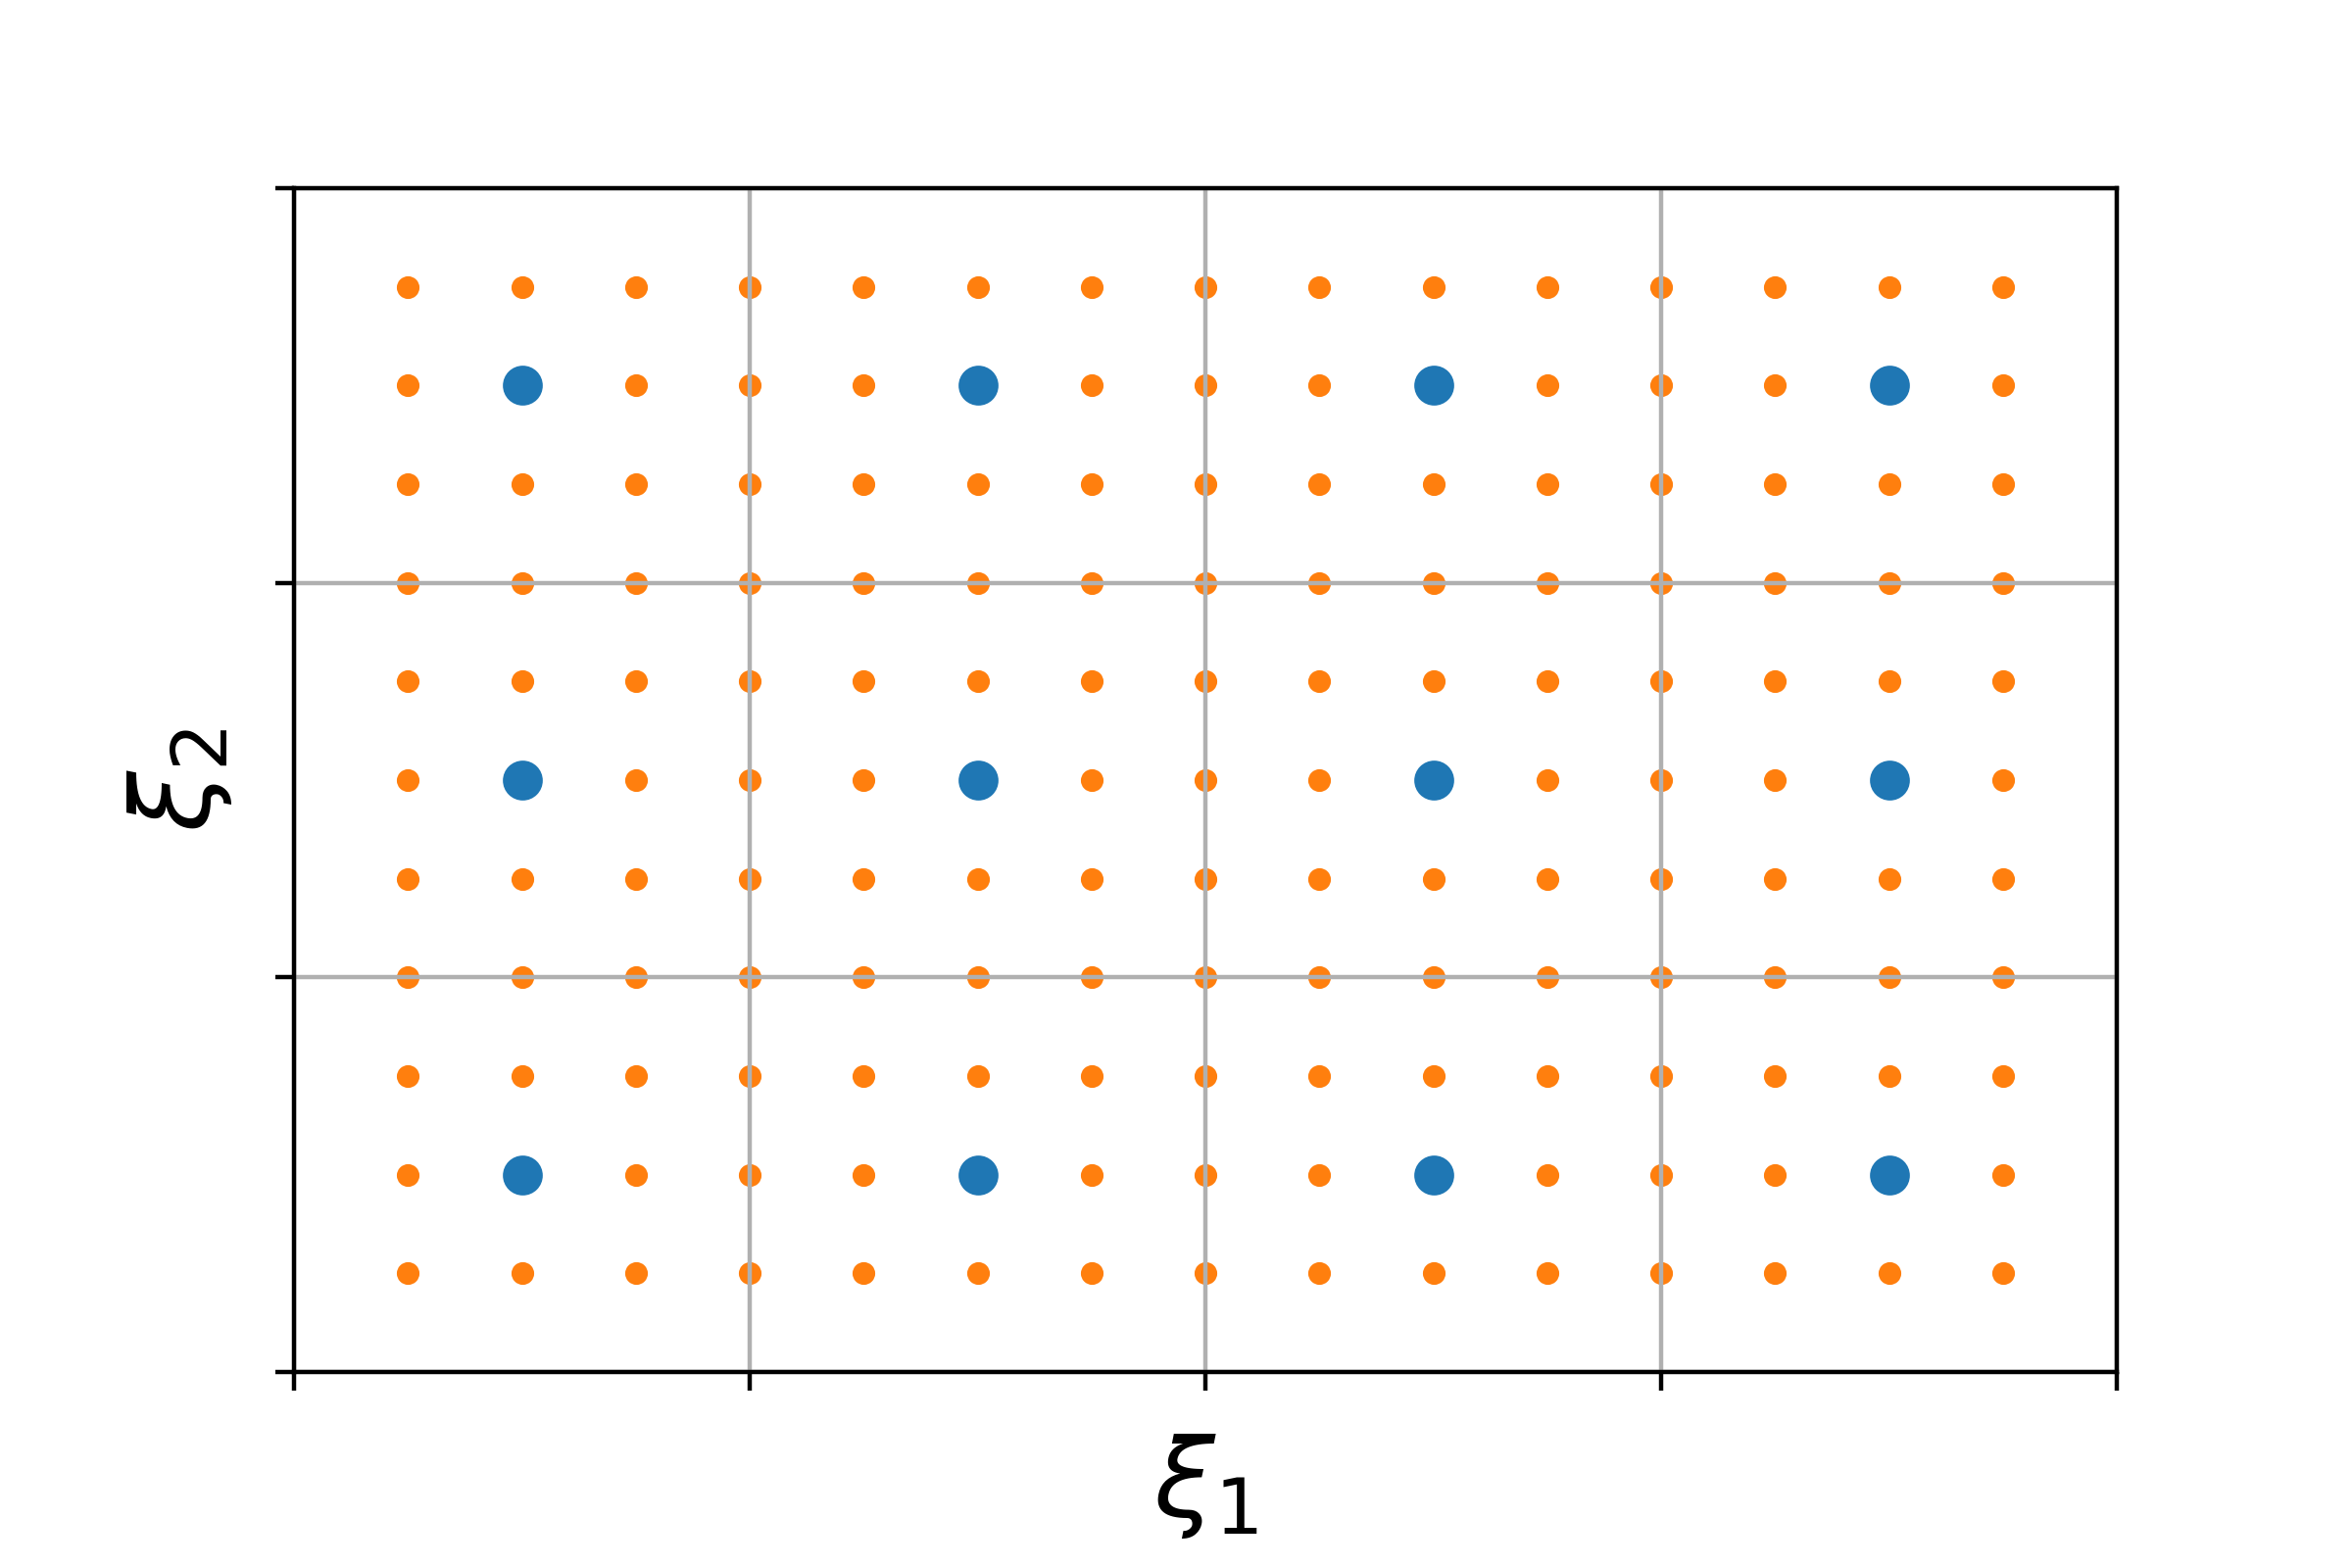
\includegraphics[width=0.49\textwidth]{bilder/grid} }}
    \caption{Illustration of the FEM method}
\label{fig:FEM}%
\end{figure}

The last missing ingredient for the ABF method now is an explicit expression for the instantaneous force samples $F_{\xi}$. Carter et al.\autocite{carter1989constrained} gave a first general expression:
\begin{equation}
  F(\xi,\textbf{q}) = -\frac{\partial V(\xi,\textbf{q})}{\partial \xi} + \beta^{-1} \frac{\partial \ln|J(\xi,\textbf{q})|}{\partial\xi} \label{eq:instforce old}
\end{equation}
which depends implicitly on a vector field $\partial x_i / \partial \xi$, hereafter referred to as "inverse gradient" and on an Jacobian correction term purely geometric in origin. The inverse gradient can be thought of as direction along which an infinitesimal change in $\xi$ is propagated in Cartesian coordinates, the complementary coordinates $\textbf{q}$ being kept constant. A major drawback of this formalism is the requirement of an full coordinate transform from Cartesian coordinates ($\textbf{x}$) to generalized coordinates ($\xi$, $\textbf{q}$).

This requirement could be lifted by den Otter\autocite{den2000thermodynamic}, who put forward the breakthrough idea that the change in $\xi$ can be propagated along an arbitrary vector field $\textbf{v}_i$ ($\mathbb{R}^{3N} \to \mathbb{R}^{3N}$), provided it satisfies some orthonormality conditions.
Extended to multidimensional reaction coordinates \textbf{$\xi$} = ($\xi_i$) and in presence of a set of constraints $\sigma_{k}(\textbf{x})=0$ these read:\autocite{ciccotti2005blue}
\begin{equation}
  \textbf{v}_i \cdot \nabla \xi_j = \delta_{ij} \label{eq:cond1}
\end{equation}
\begin{equation}
  \textbf{v}_i \cdot \nabla \sigma_k = 0 \label{eq:cond2}
\end{equation}
If all reaction coordinates $\xi_i$ are orthogonal to one another and to all constraints, $\textbf{v}_i = \nabla \xi_j/|\nabla \xi_j|^2$ is always a valid option, but not necessarily the best.
Otherwise conditions \ref{eq:cond1} and \ref{eq:cond2} can be fulfilled by orthogonalization:\autocite{ciccotti2005blue}
\begin{equation}
  \textbf{v}_i (\textbf{x}) = \frac{Q^i \nabla \xi_i (\textbf{x})}{|Q^i \nabla \xi_i (\textbf{x})|} \label{eq:ortho v}
\end{equation}
with projector $Q^i$ given by the orthonormal basis $\{\hat{n}|_{j}^{i}(\textbf{x})\}_{j\neq i}$ in the subspace spanned by $\{\nabla \xi_j (\textbf{x})|\}_{j\neq i} \cup \{\nabla\sigma_j (\textbf{x})|\}_{j=1,...,M}$:
\begin{equation}
  Q^i = \textbf{1} - \sum_{j \neq i} \hat{n}_{j}^{i}(\textbf{x}) \otimes \hat{n}_{j}^{i}(\textbf{x})
\end{equation}
Replacing the inverse gradient by vectorfield $\textbf{v}_i$, expression \ref{eq:instforce old} finally reduces to:
\begin{equation}
  F(\xi_i,\textbf{x}) = -\nabla V(\textbf{x}) \cdot \textbf{v}_i(\textbf{x}) + \beta^{-1} \nabla \cdot \textbf{v}_i(\textbf{x}) \label{eq:inst ABF force}
\end{equation}
but still involves the calculation of second derivatives in the form of the divergence of vector fields $\textbf{v}_i$.\autocite{comer2015adaptive} Analytic expressions for bend angles and torsion angles, used in the present work, are given in the appendix. However, for complicated CV's like torsion angles orthogonalization via equation \ref{eq:ortho v} becomes exceedingly tedious and impractical, significantly limiting the applicability of ABF for multidimensional reaction coordinates.

\subsection{extended Lagrangian based methods (eABF, meta-eABF, WTM-eABF)}
\label{sec:eABF}
To circumvent the technical requirements of ABF Lesage et al.\autocite{lesage2017smoothed} proposed an more flexible approach termed extended ABF (eABF), where additional coordinates $\lambda$ with mass $m_{\lambda}$, which are coupled to the reaction coordinates $\xi_i$ with harmonic potentials, are introduced. The extended system ($\textbf{x}$, $\lambda$) evolves according to Langevin dynamics in the potential
\begin{equation}
  U_{ext}(\textbf{x},\lambda_i) = U(\textbf{x}) + \frac{(\xi_{i}(\textbf{x})-\lambda_i)^2}{2\sigma_i^2}.
\end{equation}
where the mass of the fictitious particle $m_\lambda$ and the variance between extended coordinate and physical coordinate $\sigma_i^2=(\beta k_i)^{-1}$ are free parameters.
The key intuition behind eABF is, that in the tight coupling (low $\sigma$, high $k$) limit efficient sampling of $\lambda$ will result in efficient sampling of $\xi$.
Therefore, to obtain uniform sampling along $\xi$ it is sufficient to bias the dynamics of $\lambda$. The inverse gradient is chosen as zero for all physical coordinates $\textbf{x}$ and 1 for $\lambda$.
This way constraints \ref{eq:cond1} and \ref{eq:cond2} are always satisfied, which is especially useful for calculations involving a set of non-orthogonal reaction coordinates.
In practice the Langevin integrator for the extended system is implemented separately from the physical MD engine and can be coupled to any collective variable of interest without additional effort.
Sampling the extended system in thermal equilibrium gives the following Boltzmann distribution in $\lambda$:
\begin{equation}
  \rho^k(\lambda) \propto \int \e^{-\beta U_{ext}(\textbf{x},\lambda)} d\textbf{x} \\
\end{equation}
The bias on $\lambda$ is the running average over the spring force in $\lambda$-bin k:
\begin{equation}
  \overline{F}(\lambda_{i}, k) = \frac{\partial A^{k}(\lambda_{i})}{\partial \lambda_i} = \frac{1}{N_{Step}^{k}\sigma_i^2} \sum_{\mu=1}^{N_{Step}^{k}} (\lambda_{i,\mu}^{k}-\xi_{i,\mu}^{k})
\end{equation}
Note that the instantaneous force estimate in each step no longer depends on the all atomic coordinates $\textbf{x}$ like in normal ABF (cf. equation \ref{eq:inst ABF force}), but only on ($\lambda_i - \xi_i$).
This has the advantageous side effect, that the noise in $\overline{F}$ can be reduced significantly and faster convergence of $\overline{F}$ can be expected, if $\sigma^2$ is well chosen.\autocite{lesage2017smoothed} Specifically, the mean square fluctuations of the spring force is given by $\sigma_F \propto (\beta\sigma)^{-1}$, which shows that the variance of $\overline{F}$ is smaller for higher values of $\sigma$.
For small values of $N_{Step}^{k}$ the linear ramp function $R(N_{Step},k)$ given by equation \ref{eq:ramp} is used nonetheless. Overall, with the time dependent bias converging towards $A^{k}(\lambda_{i})$ the biased Boltzmann distribution converges towards:
\begin{equation}
  \tilde{\rho}^k(\textbf{x},\lambda_i) \propto \e^{-\beta U_{ext}(\textbf{x},\lambda_i) + A^{k}(\lambda_i)}
\end{equation}
We now need to find a robust estimator to recover the unbiased free energy of the physical system $A(\xi_i)$ from biased dynamics in the extended system.
The naive approach is to approximate $A(\xi_i)$ with $A^k(\lambda_i)$, which can be obtained by simply integrating the bias force $\overline{F}(\lambda_{i})$ like in normal ABF.
However, this will only produce unbiased results in the tight coupling limit for $\sigma \rightarrow 0$, where standard ABF is recovered.

However, as we saw earlier, it is advantageous to use higher values of $\sigma$.
An asymptotically unbiased estimator of the free energy can be derived by correcting the free energy gradient obtained from the eABF-biased distribution $\tilde{\rho}(z)$ with the average biasing force on z
\begin{equation}
  \frac{\partial A(z)}{\partial z_i} = -\beta^{-1}\frac{\partial \ln \tilde{\rho}(z)}{\partial z_i} + k(\braket{\lambda_i}_{z}-z_{i}) \label{eq:CZAR}
\end{equation}
which is called "Corrected z-averaged restraint" (CZAR) and can be calculated on-the-fly during the simulation at little extra cost by introducing two additional accumulators for $\tilde{\rho}(z)$ and $k(\braket{\lambda_i}_{z}-z_{i})$ which are only joined at output times.\autocite{lesage2017smoothed}

The CZAR estimator is able to recover the unbiased free energy derivative only from time trajectory $(z_i,\lambda_i)$ of the extended system, independent of the bias on $\lambda_i$, as long as the simulation is in thermal equilibrium. It is therefore possible to use any arbitrary bias on $\lambda_i$, for example using metadynamics on the extended variable (eMtd, eWTM).
One particular useful choice for $\overline{F}(\lambda_{i}, k)$ is to combine the repulsive MtD or WTM potential with the eABF bias, an idea the authors figuratively described with 'Shaving Barriers, and Flooding Valleys'.\autocite{fu2018zooming}
This way the inherent difficulty in all ABF methods to get accurate force estimates in high free energy regions at the beginning of the simulation can be solved, by pushing the system towards this regions with an repulsive potential.
The full MtD-eABF and WTM-eABF bias terms read
\begin{equation}
  F_{B}^{MtD-eABF}(\lambda_i, t) = -\frac{\braket{\xi_i(\textbf{x})-\lambda_i}_{\lambda_i}}{\beta \sigma_i^2}+\frac{\partial}{\partial \lambda_i} U_{B}^{MtD}(\lambda_i,t)
\end{equation}
\begin{equation}
  F_{B}^{WTM-eABF}(\lambda_i, t) = -\frac{\braket{\xi_i(\textbf{x})-\lambda_i}_{\lambda_i}}{\beta \sigma_i^2}+\frac{\partial}{\partial \lambda_i} U_{B}^{WTM}(\lambda_i,t)
\end{equation}
with $U_{B}^{MtD}$ and $U_{B}^{WTM}$ given by equations \ref{eq:U_mtD} and \ref{eq:WTM}.
The relative contributions of the eABF and MtD/WTM term will fluctuate over the course of a simulation, but the sum of both will eventually converge. However, accurate evaluation of $F_B$ is not even required, because it only enhances sampling of the reaction coordinate and the true PMF is obtained independently from CZAR.

\section{Obtaining reaction rate constants from biased simulations}
\label{sec:A_geom}
All methods described so far enable the efficient calculation of some CV-based FES, as defined in equation~\ref{eq:free energy}. As already noted in section \ref{sec:freeE}, this formulation is not invariant under the transformation of CV, e.g. $A(\xi(\textbf{x}))\neq A(\zeta(\textbf{x}))$. It is therefore a purely thermodynamic quantity, encoding the statistical properties of a system in thermal equilibrium, and can not be used to obtain kinetic information, like free energy barriers $\Delta^\ddagger A_{A\rightarrow B}$ or reaction rate constant $k_{A\rightarrow B}$.\autocite{bal2020free}

\begin{figure}[H]
    \centering
    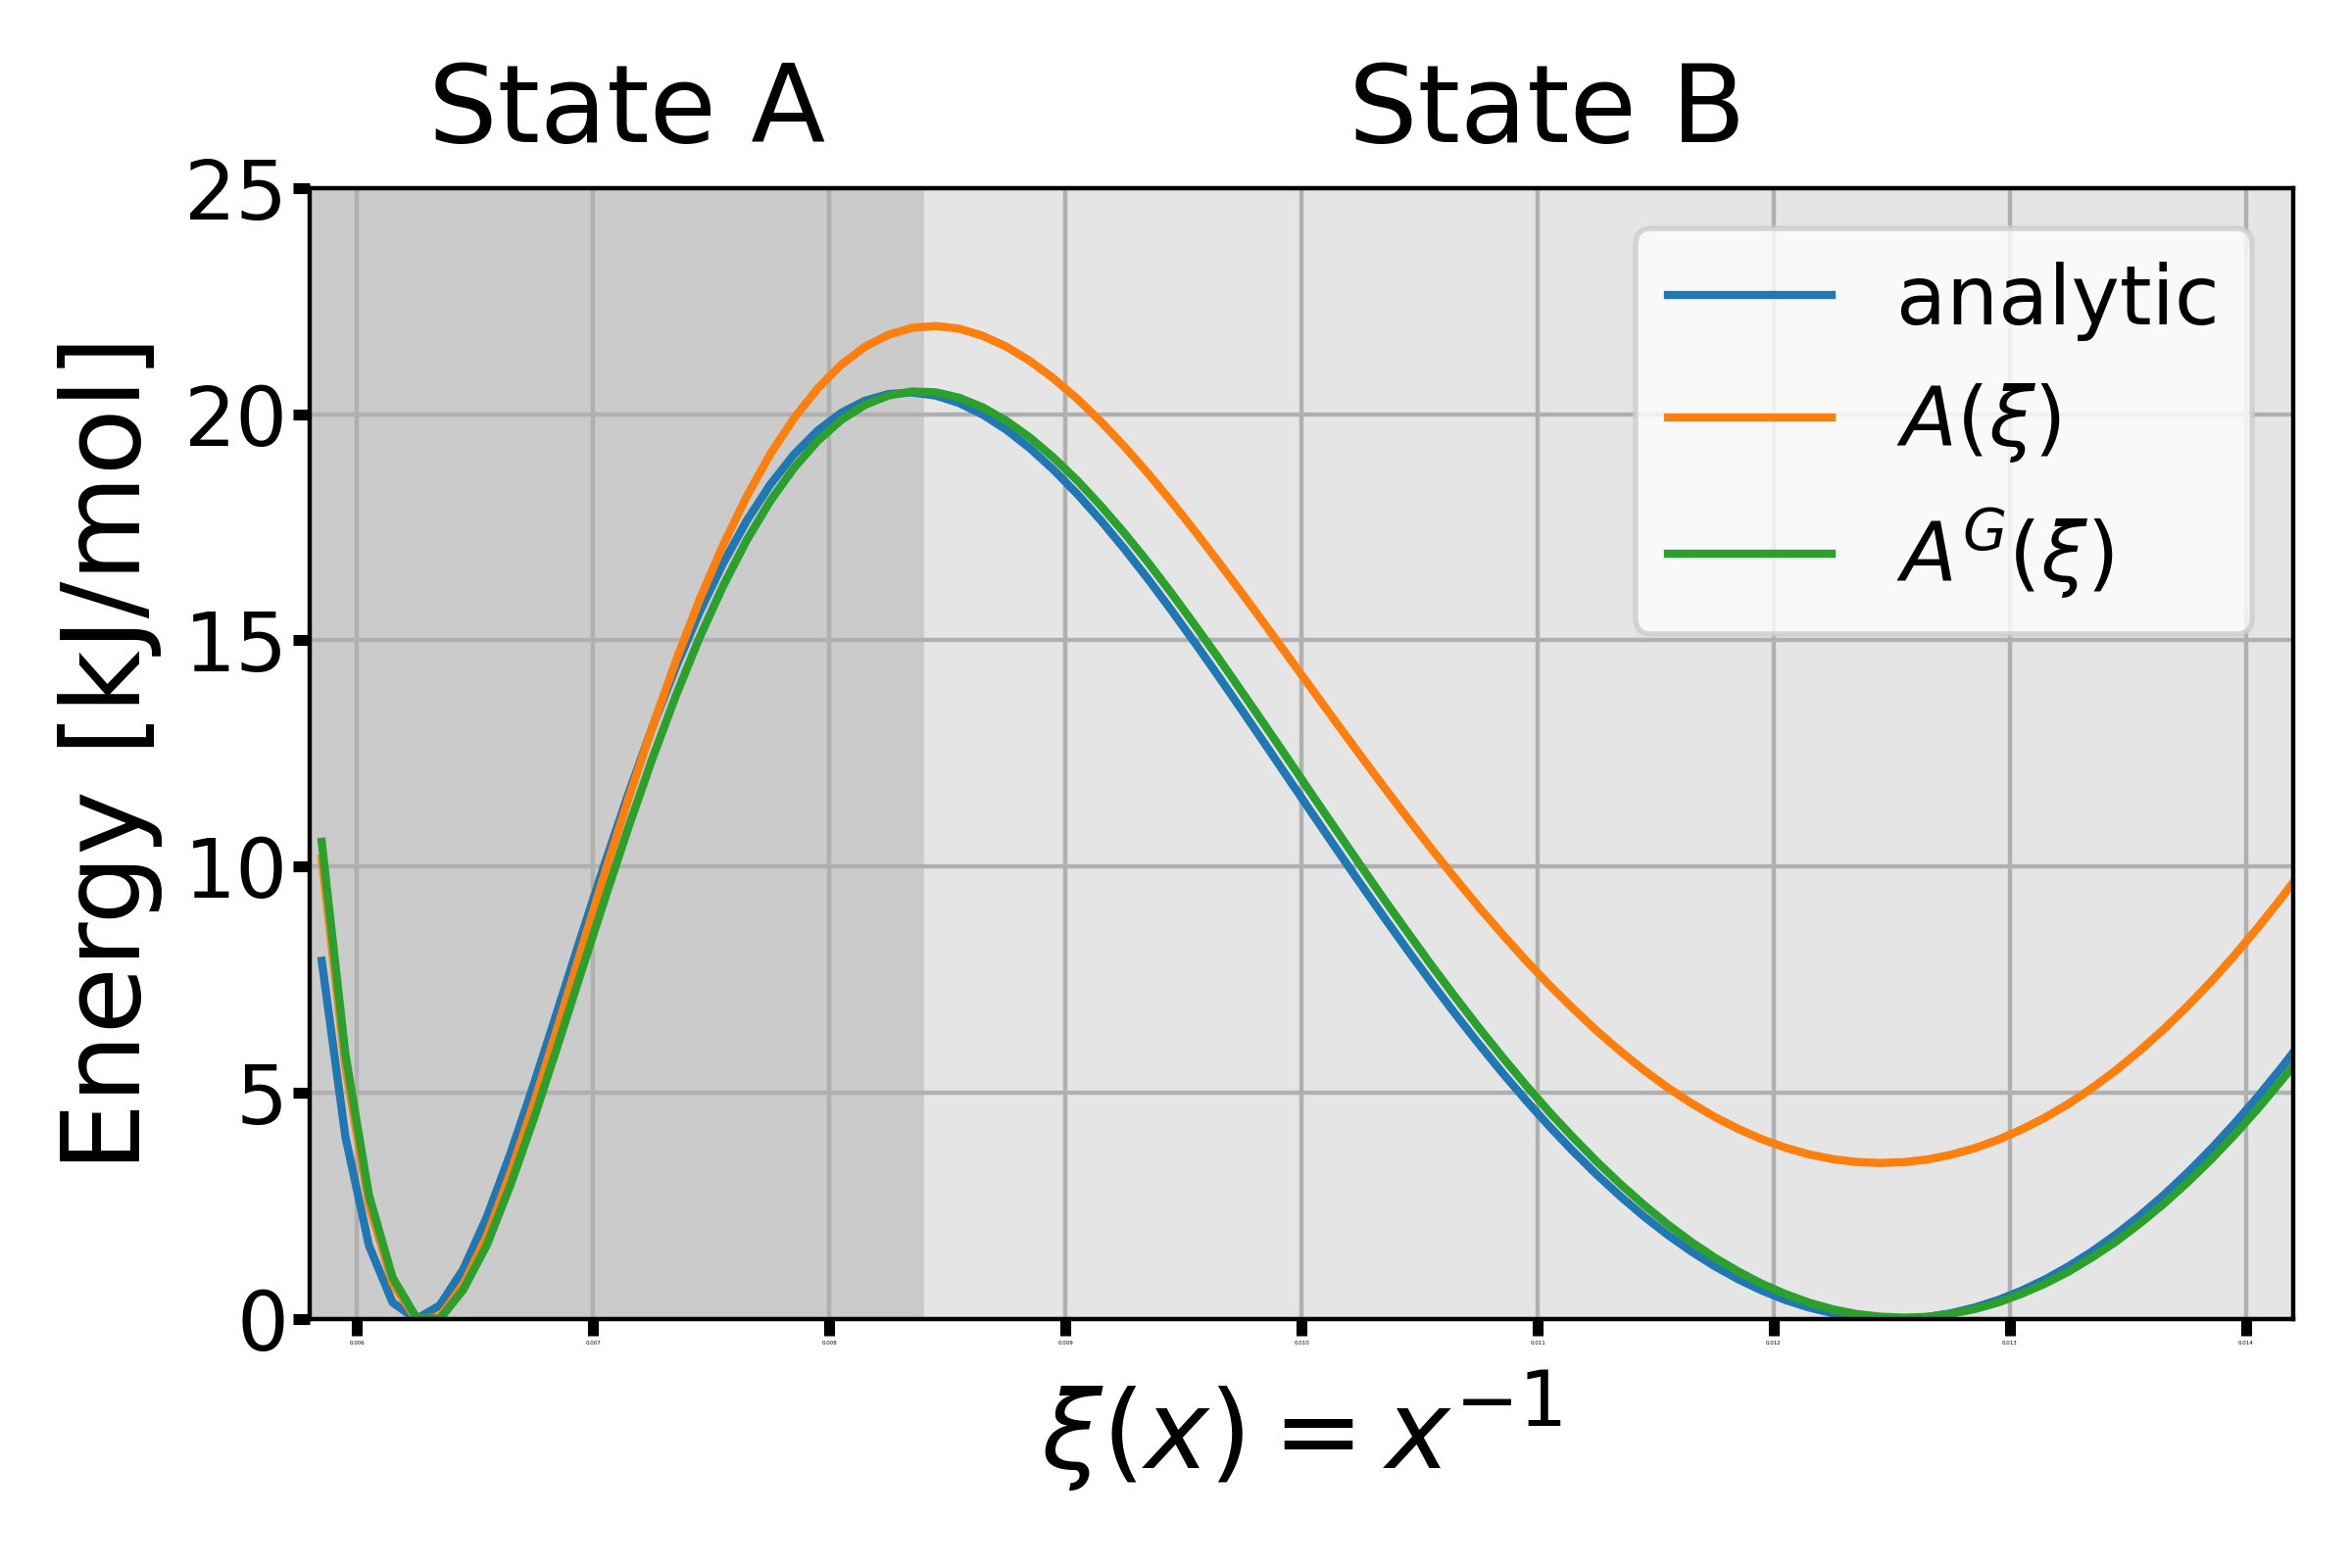
\includegraphics[width=0.6\textwidth]{bilder/geom_free_energy}
    \caption{Geometric free energy}
\label{fig:FEM}%
\end{figure}
